% !TEX root = AImath.v4.tex

\chapter{机器学习：学习如何学习？}\label{ch:机器学习}

 \begin{introduction}
  \item Definition of Theorem
  \item Ask for help
  \item Optimization Problem
  \item Property of Cauchy Series
  \item Angle of Corner
\end{introduction}

A computer program is said to {\em learn} from experience~$ E$ with respect to some class of tasks~$T$ and performance measure~$P$, if its performance at tasks in~$T$, as measured by~$P$, improves with experience~$E$.

机器学习是对能通过经验自动改进的计算机算法的研究：对于一个计算机程序，给它一个任务~$T$和一个性能测量方法~$P$，如果在经验~$E$的影响下，~$P$对~$T$的测量结果得到改进，那么就说该程序从~$E$中学习。
\begin{flushright}
— Tom M. Mitchell  [1997]
\end{flushright}

人工智能从诞生至今，经历了一次又一次的繁荣与低谷，其发展历程大体上可以分为“推理期”，“知识期”和“学习期”%\cite{周志华, 2016}。\cite{WangJue2006MachineLearning}。

%在人工智能半个世纪多的发展过程中，经历了两大阶段：
%首先是自上而下阶段，由人工建立规则，在此基础上进行逻辑推理和知识库构建。主要代表是符号主义学派。 
%
%后来发展为自下而上的从经验、反馈中自主学习，这包括机器学习与深度学习的联结主义学派，以及以机器人为代表的行为主义学派。
%
%即从推理期和知识期，走向学习期。 
%
%人工智能的发展经历了显著的转型：从依赖人工规则的符号主义学派，到借助经验和反馈的联结主义与行为主义学派，AI的核心方法从“推理期”和“知识期”逐渐过渡到“学习期”。这种变化反映了AI在应对复杂问题时，从自上而下的规则构建转向自下而上的经验学习。符号主义学派强调人工设计规则和知识库来解决问题，而联结主义学派和行为主义学派则更关注如何通过数据驱动的方式从经验中学习知识。

你可能已经接触过编程，甚至开发过一些程序。同时，你或许也读过关于深度学习或者机器学习的铺天盖地的报道，尽管这些技术常常被赋予了更广义的名字“人工智能”。实际上，或者说幸运的是，大部分程序并不需要深度学习或者广义的人工智能技术。
例如，为微波炉设计一个用户界面时，我们只需简单设置几个按钮，并编写规则来精确描述微波炉在各种情况下的表现。
再比如，设计一个电子邮件客户端，虽然复杂一些，但仍可以通过逻辑来实现：创建输入框接收收件人、主题和正文，监听用户输入，并在“发送”按钮被点击时检查邮箱格式和主题内容，再通过协议发送邮件。

这些例子表明，很多常见程序的实现并不依赖真实世界的数据，也不需要从数据中提取特征。只要有足够的常识和编程技巧，我们就可以通过逻辑和规则完成这些任务。

事实上，符号主义AI是是AI发展的第一阶段。
在人工智能半个多世纪的发展历程中，符号主义AI曾主导数十年。通过人工设定规则和逻辑推理，符号主义AI为解决复杂问题提供了切实可行的框架，推动了专家系统和符号推理模型在多个领域取得成果。符号主义AI的典型方法，如博弈树和专家系统中的推理，擅长解决规则明确的问题。

然而，随着应用需求的拓展，符号主义的局限性逐渐显现：人工规则难以精确描述复杂的现实场景，知识工程的构建过程费时费力且难以扩展，特别是在面对海量、非结构化数据时，手工设定规则既低效，又难以有效应对。
这种局限性催生了对新的自动化学习方式的需求。

\section{机器学习，必然选择}
%\cite{机器学习波澜壮阔40年2018}

我们很容易就能找到一些即使是世界顶尖的程序员也无法仅凭编程技巧解决的问题。这些问题的共同特点在于它们“只可意会而难以言传”：对于人类而言，这些任务似乎轻而易举，但要解释我们是如何做到的却并不简单---很难明确地描述出其中的规则和细节。这些特性使得依靠人工设计程序来解决此类问题变得困难重重。

\begin{figure}[htbp]
\centering
\begin{minipage}{0.4\linewidth}
\centering
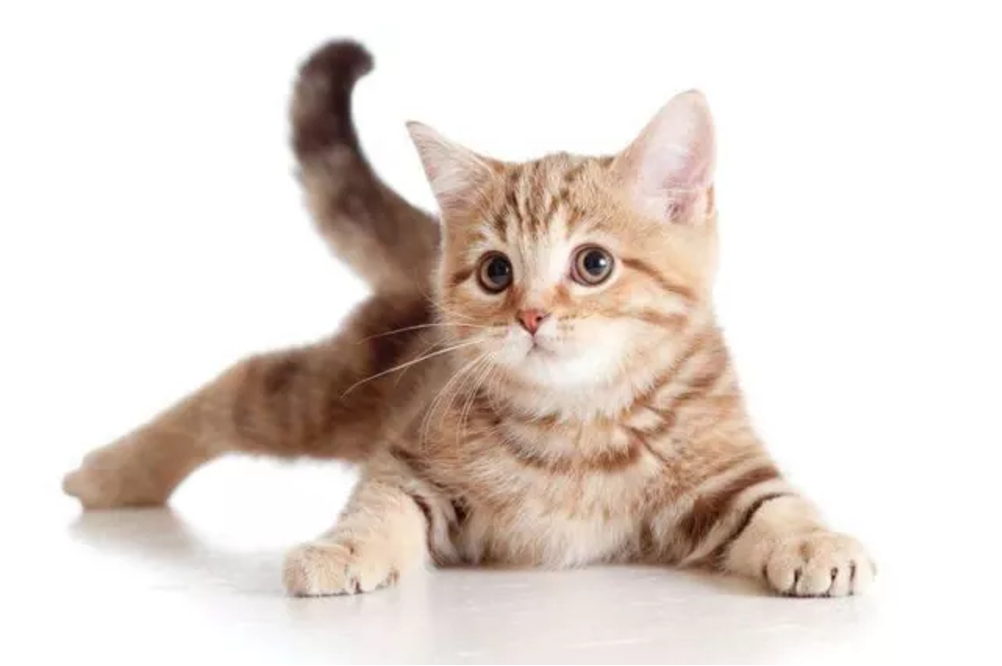
\includegraphics[width=0.9\linewidth]{figs/猫.png}
\caption{识别“猫”}
\label{识别“猫”}%文中引用该图片代号
\end{minipage}

\begin{minipage}{0.4\linewidth}
\centering
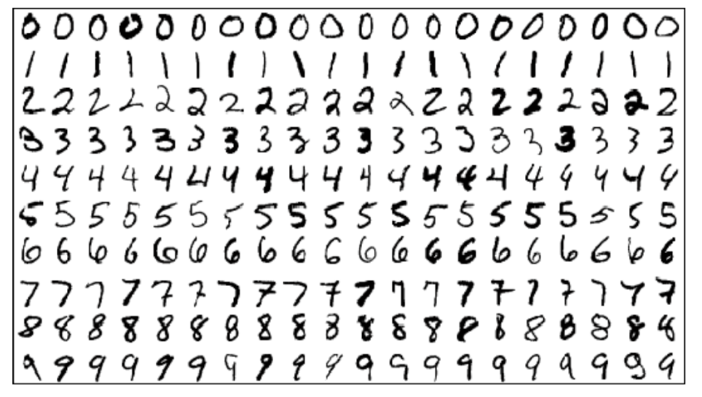
\includegraphics[width=0.9\textwidth]{figs/手写数字识别.png}
\caption{手写数字识别(图片来源~\cite{lecun1998gradient})}
\label{手写数字识别1}
\end{minipage}
\end{figure}

假设我们希望开发一个程序来识别图~\ref{识别“猫”}中有没有猫。这个问题对于我们来说非常简单，正常视力的人都能一眼分辨。
然而，如果要基于规则和编程来实现这一判定，任务复杂得难以想象， 甚至曾让顶尖的计算机科学家和程序员感到棘手。

在符号主义AI的框架下，我们需要手动定义规则来描述“猫”的特征，比如毛发分布、耳朵形状、眼睛大小、尾巴形状等。实际上，要判断图像中是否有猫，必须结合成千上万像素的特征，如边缘、质地、形状，甚至是眼睛和鼻子的具体细节。
但这种方法对复杂图像来说几乎不可行。以一张$512 \times 512$像素的黑白图像为例。每个像素取值在0到255之间，那么所有可能的像素组合多达$256^{512\times 512}=256^{262144}$种。这样的天文数字，即便在当今的计算能力下也难以实现。
更复杂的是，不同图像中的猫在姿态、颜色、角度、光线和背景等方面可能千差万别。因此，为猫的所有可能形态设计一套完备的规则几乎不可能。

我们再来看另一个例子---手写体数字识别。手写数字识别\cite{lecun1989backpropagation}是一个经典的机器学习任务，对人来说很简单，但对计算机而言却十分困难。
不同人书写的数字风格和特征各异。比如，数字“5”的形状在不同书写习惯下变化多端，笔画粗细、弯曲程度和角度均不相同。
要编写一套基于规则的算法来识别数字“5”，几乎无法穷尽所有可能的变化。
类似地，其他手写数字的多样性和变形空间，使得基于人工规则来识别这些数字成为一项无法完成的任务。

在现实生活中，很多问题如人脸识别、物体识别、语音识别等，都和猫的识别、手写体数字识别一样，属于“只可意会不可言传”的温特，难以通过穷尽特征规则来精确完成，即使结合一些启发式规则，其过程也极其复杂。因此，基于符号规则的方法并不适合解决这些"“意会难传”的任务。
因此，AI需要一种能够自动提取规律的学习方式。

\subsection{机器学习：从数据中学习规律}
一种解决以上问题的思路是逆向思考：与其设计繁琐的规则去定义“猫”的特征，不如从最终的需求入手，尝试“用数据编程”。通过将大量样本数据“喂给”模型，让模型自动提取出共性和模式，从而实现自动化学习。

以“猫的识别”为例，我们可以收集大量已知包含猫和不包含猫的图像，模型通过这些样本的训练后，能够找到模式并生成一个函数，用于判断图像中是否包含猫。这个函数的形式可以因问题的不同而变化：它可能是简单的二次函数，也可能是复杂的神经网络模型，而其具体参数则通过数据自动确定。
类似的过程也适用于手写体数字识别等任务。为了让计算机识别手写数字，我们可以准备大量带标注的手写体数字图像作为训练数据，通过学习算法，模型会生成一套识别规则，用于识别新的手写体数字。

这一基于数据自动优化函数参数的过程，正是机器学习的本质：让计算机从数据中学习规律。

\section{机器学习是什么？}\label{sec:机器学习}

Arthur Samuel (1959) 将机器学习定义为：
“Field of study that gives computers the ability to learn without being explicitly programmed”
在不针对计算机编程的情况下，赋予计算机学习能力的一个领域。

{\em (有重复，需润色)著名学者赫伯特\textperiodcentered 西蒙教授（Herbert Simon，1975年图灵奖获得者、1978年诺贝尔经济学奖获得者）曾对“学习”下过一个定义：“如果一个系统，能够通过执行某个过程，就此改进了它的性能，那么这个过程就是学习”。言简意赅，一针见血。从西蒙教授的观点可以看出，学习的核心目的就是改善性能。

遵循西蒙教授的观点，对于计算机系统而言，通过运用数据及某种特定的方法（比如统计方法或推理方法）来提升机器系统的性能，就是机器学习（Machine Learning，简称ML）。

英雄所见略同。1997年，卡耐基梅隆大学的机器学习和人工智能教授汤姆\textperiodcentered 米切尔（Tom M. Mitchell），在他的经典教材《机器学习》\cite{mitchell1997}中，也给出了一个更为具体（其实也很抽象）的定义：

“A computer program is said to {\em learn} from experience~$ E$ with respect to some class of tasks~$T$ and performance measure~$P$, if its performance at tasks in~$T$, as measured by~$P$, improves with experience~$E$”

（对于一个计算机程序，给它一个任务(Task，简称~$T$)和某种性能度量准则(Performance，简称~$P$)，如果随着经验(Experience，简称~$E$)的积累，~$P$对~$T$的度量结果得到改进，那么称这个计算机程序从经验~$E$中进行了学习。)

比如，学习围棋的程序AlphaGo，它可以通过和自己下棋获取经验，那么，它的任务T就是“参与围棋对弈”，它的性能P就是用“赢得比赛的百分比”来度量的。类似的，学生的任务T就是“上课看书写作业”，它的性能P就用“考试成绩”来度量。

因此，Mitchell教授认为，对于一个学习问题，我们需要明确三个特征：任务的类型、衡量任务性能提升的标准以及获取经验的来源。

事实上，看待问题的角度不同，机器学习的定义也略有不同。比如，支持向量机（SVM）的主要提出者弗拉基米尔\textperiodcentered 万普尼克（Vladimir Vapnik），在其著作《统计学习理论的本质》\cite{vapnik2000统计学习理论的本质}中就提出，“机器学习就是一个基于经验数据的函数估计问题”。
而在另一本由斯坦福大学统计系的特雷弗\textperiodcentered 哈斯蒂（Trevor Hastie）等人编写的经典著作《统计学习基础》\cite{hastie2015} 则认为，机器学习就是“抽取重要的模式和趋势，理解数据的内涵表达，即从数据中学习（to extract important patterns and trends, and understand “what the data says. We call this learning from data）”。
这三个有关机器学习的定义，各有侧重，各有千秋。Mitchell的定义强调学习的效果；Vapnik的定义侧重机器学习的可操作性；而Hastie等人的定义则突出了学习任务的分类。但其共同的特点在于，都强调了经验和数据的重要性，都认可机器学习提供了从数据中提取知识的方法。

当下，我们正处于大数据时代。众所周知，大数据时代的一个显著特征就是，“数据泛滥成灾，信息超量过载，然而知识依然匮乏不堪”。因此，能自动从大数据中获取知识的机器学习，必然会在大数据时代的舞台上扮演重要角色。}

机器学习(Machine Learning，ML)，顾名思义，机器具备有学习的能力。更具体地，机器学习是指让计算机从数据中进行自动学习，得到某种知识或规律，然后利用学习到的规律(模型)对未知或无法观测的数据进行预测。机器具备学习能力之后，可以做很多事。比如下棋、图像识别、语音识别等等。

机器学习和普通程序的一个本质区别是需要样本数据，是一种数据驱动的方法。这种“用数据编程”的方法论构成了当今机器学习和深度学习的核心思想。

事实上， 这种方式与人类的学习过程十分相似：教小孩认识物品和数字时，我们也是通过展示大量实例帮助他们从中总结规律。同样，计算机通过“看”大量样本，从中学习特征，再利用这些特征识别新的样本。

面对规则难以解决的任务，机器学习成为了一个自然的选择。这种自下而上通过数据驱动自动学习和优化参数的方法，使得模型能够适应更为复杂的环境和动态任务。

无论是猫和手写数字的识别，还是更为复杂的语言和视觉生成任务，机器学习都展现了符号主义AI无法比拟的灵活性。
随着数据量和计算能力的提升，机器学习逐渐取代了早期的规则定义方法，广泛应用于模式识别、预测等领域，已成为人工智能发展的重要基石。
伴随着方法论的突破以及计算资源和数据量的提升，机器学习在1980年代之后逐渐取代符号主义，成为AI的主流。机器学习不仅拓展了AI的应用范围，还为现代AI在图像识别、自然语言处理等领域的应用奠定了坚实基础。

%机器学习问题在早期的工程领域也经常称为模式识别(Pattern Recognition，PR)，但当时的模式识别更偏向于具体的应用任务，比如光学字符识别、语音识别，人脸识别等。这些任务的特点是对于我们人类而言，这些任务很容易完成，但我们不知道自己是如何做到的，因此也很难人工设计一个计算机程序来解决这些任务。

\section{机器学习：寻找一个函数}
机器学习的过程实际上是“寻找一个函数”，即学习一个映射~$f: X \rightarrow Y$， 以描述输入~$X$与输出~$Y$之间的关系，如图~\ref{机器学习：寻找一个函数} 所示。

机器学习的核心在于构造映射，这一原则贯穿了不同的应用场景：

无论是传统的 AI 应用（如机器翻译、图像识别），还是如今大热的生成式模型（如“文生文”、“图生文”、或“语音生文本”等），其核心都是在构建一个函数，将不同类型的输入映射为对应的输出。
例如，
\begin{itemize}
\item {\bf 图像分类：} 模型通过学习图像的像素特征，找到一个函数，将其映射到相应的分类标签，最终输出准确的结果。 
\item {\bf 机器翻译模型：} 将一句话映射到另一种语言下的等义句
\item {\bf 语音识别：} 输入是声音信号，输出是对应的文字内容。语音识别的函数需要将连续的语音信号转化为离散的文本信息，这一映射极为复杂，人类难以直接手工定义。
\item {\bf  图像识别：} 输入是一张图片，输出是这张图片中的内容（如分类标签或对象名称）。这一函数需要捕捉像素间的复杂关系来识别图像中的模式。
\item {\bf 围棋对弈：} 以 AlphaGo 为例，这里的函数输入是棋盘上黑白子的位置分布，输出是机器下一步的最佳落子位置。这个函数需要从海量的棋谱中学习策略，评估每种可能的走法。
\item {\bf 文本生成文本：} 如大语言模型（LLM），通过训练大量文本数据，实现从语言到语言的映射，如回答问题、生成摘要等。 
\item {\bf 图像生成文本：} 在图像描述任务中，模型通过对图像的分析将图像转化为文本描述，实现“图像到语言”的映射。这个映射函数训练的核心是让模型能够从图像中提取特征，将图像的关键信息通过自然语言表达出来。
\item {\bf 文本生成图像：}文本生成图像（如DALL-E）将描述性文本转化为图像，是一个“文字到图像”的映射过程，这种映射往往需要处理大量语言和视觉信息的复杂关联。
\item {\bf 语音生成语音：} 语音识别和合成是通过分析音频特征生成文字或合成语音，实质是语音到语音的映射函数。
\item {\bf 大模型：} 即使是复杂的生成式大模型，如 ChatGPT 或 DALL-E，依然是在文本和图像之间构建映射关系：从用户输入的文本生成合适的回答或图像，这些映射关系都来源于对数据关联的学习。
\end{itemize}
这些映射任务依赖于深度学习中的神经网络，通过多层神经网络捕捉数据之间的深层模式，处理复杂的输入与输出关系。

因此，所有这些任务背后的共性是，它们都需要一个极为复杂且难以手工定义的函数来描述输入与输出的关系。
最终的任务都是在“寻找一个函数”——即在已知的输入与期望的输出之间找到最合适的映射关系：
{\em 通过一个学习算法(learning algorithm)~$\mathcal{A}$，在训练集上找到一组参数~$\theta^\ast$， 使得函数~$f({\bf x}, \theta^\ast)$可以近似真实的映射关系。这个过程称为学习(learning)或 训练(training)过程，函数~$f({\bf x}, \theta)$ 称为模型(model)。}

机器学习通过大量标注好的输入和对应的输出（样本）的训练，自动构建这个映射函数，以最小化预测结果与真实标签之间的误差为目标，不断迭代优化模型参数，从而将输入转化为期望的输出。最终，模型不仅在训练数据上表现良好，还能在新样本上有较强的泛化能力，从而实现准确的预测或分类。

\begin{figure}[htbp]
\centering
\begin{subfigure}{0.49\linewidth}
\centering
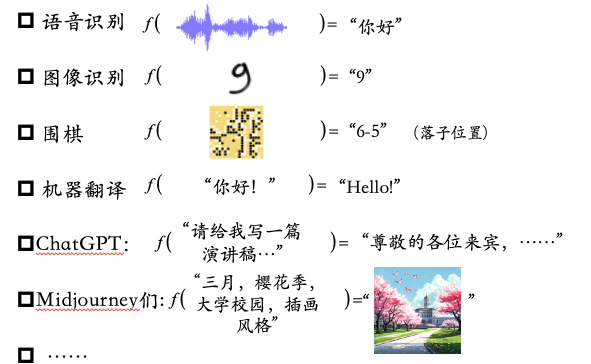
\includegraphics[width=1\linewidth]{figs/机器学习=一个函数.png}
\caption{机器学习$\sim$寻找一个函数}
\label{机器学习}
\end{subfigure}
\begin{subfigure}{0.49\linewidth}
\centering
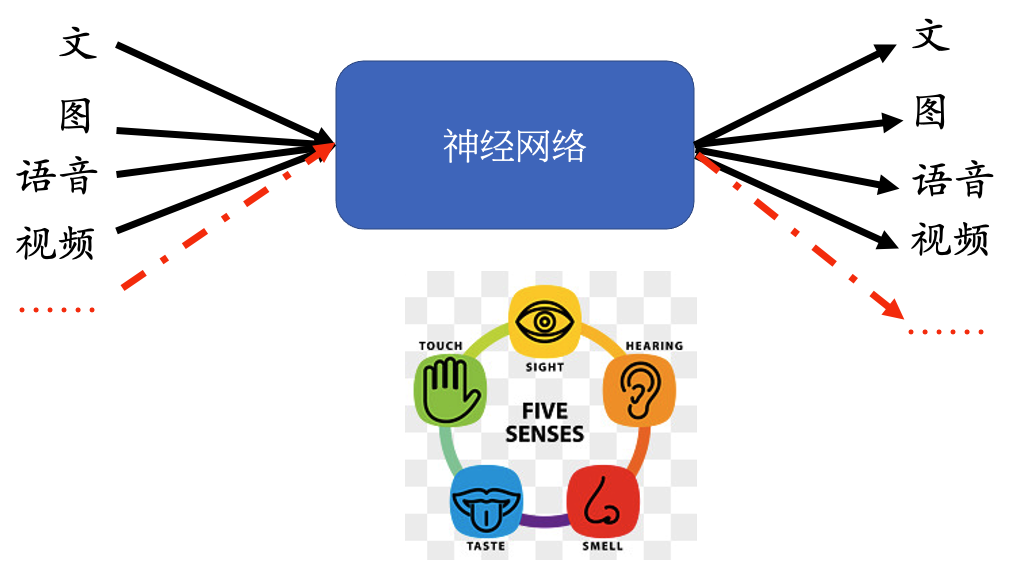
\includegraphics[width=1\textwidth]{figs/LLM函数.png}
\caption{主流的LLM应用}
\label{LLM映射}
\end{subfigure}
\caption{机器学习$\simeq$寻找一个函数}
\label{机器学习：寻找一个函数}
\end{figure}

\footnote{事实上，从更广义的角度看，不仅机器学习，符号主义AI乃至整个数学科学研究都是在寻找某种映射或函数。无论是符号主义AI中的逻辑推理，还是数学运算的算法设计，本质上都是在构建映射，将输入转化为理想的输出结果。

在符号主义AI中，人工构建的规则或知识库即为映射的载体。例如，通过逻辑规则构建推理引擎，输入一些前提条件后，系统可以推导出结论；这种推理过程就是一种映射，将输入事实映射到可能的结论。

数学中的很多经典算法同样是映射的体现。例如，辗转相除法是一种将两个整数映射到它们最大公因子的函数，归结起来是一系列除法操作的映射过程。类似地，求解一元二次方程、最小公倍数等，都可以被看作是将特定输入映射到对应结果的算法。

这种“寻找映射”的思想不仅贯穿于AI和数学，更广泛地延伸到科学的其他领域。从本质上说，科学研究的很多过程也在尝试通过公式、定理、模型等将实验条件与结果进行关联，使得我们能够从已知条件出发预测或解释未知现象。这也正是科学和技术的核心追求：构建从数据、规律到结果的高效映射，将复杂的现实问题简化为可以求解的模型。}

\begin{figure}[htbp]
\centering
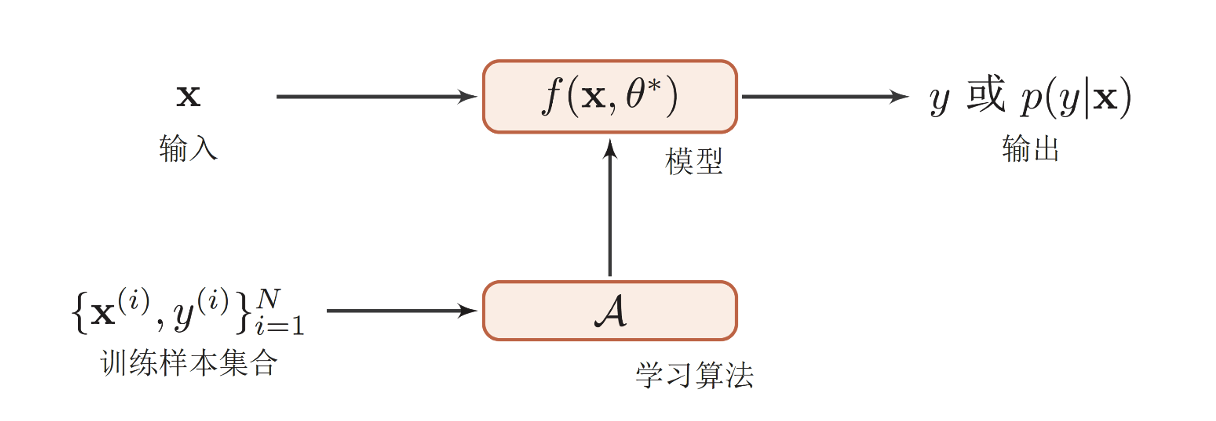
\includegraphics[width=1\textwidth]{figs/机器学习-构造一个函数.png}
\caption{机器学习-构造一个函数}
\label{机器学习-构造一个函数}
\end{figure}

\subsection{数据驱动的函数优化}
事实上，从更广义的角度看，不仅机器学习，符号主义 AI 乃至整个数学研究都是在寻找某种映射或函数，将输入转化为理想的输出结果。例如，用于诊断血液感染的医疗专家系统 MYCIN，即是通过一系列推理规则将患者症状映射到可能的疾病诊断和治疗方案。

然而，与符号主义 AI 不同的是，机器学习并不依赖人工定义的规则，而是通过数据驱动的方式自动寻找映射函数。
通常，机器学习算法首先选择一个合适的模型结构（例如线性回归、决策树、神经网络等）来表达输入 $X$ 和输出 $Y$ 之间的关系，通过大量标注样本数据的训练不断优化模型参数，使得输出尽可能接近目标。
%模型的目标是识别数据间的深层模式，从而在实际以你该用中能够合理地预测或生成输出。

在机器学习中，“寻找函数”并非直接写出公式，而是让机器通过优化算法自行找到尽可能最佳的近似映射。
无论是线性回归、支持向量机、神经网络还是深度学习模型，核心都是利用大量数据训练出一组参数，使得模型在新样本上也能表现良好。
%这一训练过程实质上是优化函数，使得输出尽可能接近目标。

\subsection{ 挑战：找到一个精准的函数}
“寻找一个函数”听起来很直观，但在复杂应用中，找到这一映射并不容易。现实世界的输入 $X$ 和输出 $Y$往往包含大量的噪声和多样性，使得找到普适的映射函数异常困难。例如，图像生成文本的模型不仅要识别出图像中的物体，还需捕捉上下文关系。类似地，在文本生成图像的任务中，则要从语言描述中理解意图并生成符合要求的图像。即便是同样的输入文本，也可能会对应到多种不同的视觉表现形式。
这些任务要求模型具备高度的抽象和泛化能力，能够在不完美的数据中找到模式，确保它对新数据同样适用。
这些任务

这种“映射的难题”也带来了多样化的模型结构和优化算法，不同的模型结构被引入以解决特定问题。比如卷积神经网络（CNN）在图像处理中的应用、递归神经网络（RNN）和自注意力机制（Transformer）在序列数据中的应用等。这些模型的共同目标是优化映射函数，使模型更好地理解输入与输出的关系。

\subsection{机器学习的未来：构建更灵活的映射函数}
未来，随着计算能力的提升和模型设计的改进，机器学习将支持更复杂的多模态映射，推动AI系统在文本、图像、语音等多种数据形式间灵活转换。无论是自动驾驶、智能医疗，还是多模态智能系统，核心任务始终是构建更高效、精确的映射函数。

随着机器学习和深度学习的发展，“寻找一个函数”这一任务上正不断迈向新的高度。从单一的输入输出模式到复杂的多模态映射，未来的AI系统或将实现文本、图像与语音之间的无缝转换，从而构建出真正多功能的智能系统。

\section{机器学习三要素：模型、学习准则、优化}

Mitchell教授认为，对于一个
机器学习的核心任务是从数据中寻找一个映射函数，将输入转化为期望的输出。对于一个学习问题，我们需要明确三个特征：任务的类型、衡量任务性能提升的标准以及获取经验的来源。

需要围绕{\bf 模型}、{\bf 学习准则}和{\bf 优化}这三个关键要素展开工作。这三者共同构成了机器学习算法的理论基础和实践框架。

\subsection{模型：映射关系的表示}

在机器学习中，模型是机器学习中的核心，它具体定义了输入数据与输出预测之间关系的数学结构，形如映射~$f: X \rightarrow Y$。
为了定义映射~$f: X \rightarrow Y$，一个机器学习任务要先需要确定其输入空间~$X$和输出空间~$Y$，不同机器学习任务的主要区别在于输出空间不同。在分类、回归、生成等不同任务中，模型的类型和结构也有所差异。在两类分类问题中~$Y = \{+1,-1\}$，在~$K$类分类问题中$Y =\{1, 2,\dots , K\}$；在回归问题中~$Y = \mathbb{R}$；而在图像生成文本（如图像描述）任务中，输入空间为图像特征，通常表示为高维张量~$X=\mathbb{R}^{H\times W\times C}$，其中，$H$ 是图像的高度，${\bf w}$ 是宽度，$C$ 是通道数（通常为~$3$，表示RGB通道），而输出空间为描述图像的自然语言文本序列~$\{y_1,y_2,\dots, y_m \}, y_j\in \mathcal{V}$。

常见的模型可以分为线性模型和非线性模型两种。线性模型的形式如下：
$$
f({\bf x}; \theta)= {\bf w}^T{\bf x} +b, 
$$
其中，~${\bf x}$为输入向量，参数~$\theta$ 为包含权重向量~${\bf w}$和偏置~$b$的可学习参数。

广义的非线性模型可以写为多个非线性基函数~$\phi({\bf x})$ 的线性组合
\begin{equation*}\label{ref}
f({\bf x}; \theta) = {\bf w}^T {\bf \phi}({\bf x}) + b, 
\end{equation*}
其中，~$\phi({\bf x}) = [ \phi_1({\bf x}),\phi_2({\bf x}),\dots ,\phi_K({\bf x})]^T$ 为~$K$个非线性基函数组成的向量，参数~$\theta$为包含权重向量~${\bf w}$ 和偏置~$b$的可学习参数。

如果~$\phi({\bf x})$本身为可学习的基函数，比如
\begin{equation*}
\phi_k(x) = h({\bf w_k}^T\phi^\prime({\bf x}) + b _k), \forall 1 \le  k \le K,
\end{equation*}  
其中，~$h(\cdot)$ 为非线性函数，~$\phi^\prime ({\bf x})$ 为另一组基函数，${\bf w}_k$ 和~$b_k$ 为可学习的参数，则~$f ({\bf x};\theta)$ 就等价于神经网络模型。

模型通过一组参数来描述这一映射关系，并通过训练过程学习这些参数的最优值。在上面的表达式中，模型可以看作是映射函数 $f$ 的候选集合，例如 $f ({\bf x};\theta)$ 表示带有参数 $\theta$ 的模型。在训练过程中，模型的目标是通过优化参数 $\theta$ 来学习数据中的规律。

模型的选择通常取决于任务的复杂性和数据的特性。不同类型的模型适应不同的任务和数据结构。
%例如，对于线性关系的任务，可以选择{\bf 线性回归}或{\bf 支持向量机（SVM）}；
%对于复杂非线性关系的任务，通常采用{\bf 神经网络}或{\bf 深度学习模型}。

{\bf 1.线性模型}

线性模型是一类假设输入特征与输出之间存在线性关系的模型。线性模型简单易懂，计算效率高，通常用于回归和分类任务。常见的线性模型包括：
\begin{itemize}
\item {\bf 线性回归：} 用于回归问题，假设目标变量与特征之间存在线性关系:
$$
y =w_1x_1+\cdots+ w_nx_n+b
$$
其中，~$w_1,\dots, w_n$是模型的权重，~$x_1,\dots,x_n$是输入特征，~$b$是偏置项。
线性回归通过最小化均方误差（MSE）来优化模型参数，广泛应用于预测问题，如房价预测、销量预测等。

\item  {\bf 逻辑回归：}用于二分类问题，尽管名字中有“回归”，但逻辑回归实际上是一个分类模型。它通过一个S型的逻辑函数（sigmoid函数）将线性输出转化为概率值，用于判定样本属于某个类别的概率:
$$
P\{ y=1 |x\} = \frac{1}{1+e^{-z}} \quad \mbox{其中} z =w_1x_1+\cdots+ w_nx_n+b
$$
这里，~$z$为线性模型的输出，~$P\{ y=1 |x\} $为预测为类别~$1$的概率。
逻辑回归广泛应用于金融风控、医学诊断等领域。
\end{itemize}
线性模型的优点是计算效率高、实现简单，但它们的局限性在于只能建模线性关系，无法处理复杂的非线性问题。

{\bf 2.树模型}

树模型是一类基于树结构进行决策的模型，适用于分类和回归问题。树模型的基本思想是通过一系列的决策规则将数据划分成不同的类别或预测值。常见的树模型包括：

\begin{itemize}
\item  {\bf 决策树（Decision Tree）：} 是一种树状结构的模型，通过一系列的条件判断（特征值划分）来预测结果。每个叶节点代表一个类别或预测值，内部节点代表特征的划分。决策树易于理解和可视化，但容易出现过拟合。典型算法包括CART（Classification and Regression Trees）。

\item  {\bf  随机森林（Random Forest）： }是一种集成学习方法，通过构建多颗决策树并结合它们的预测结果来提高模型的准确性和泛化能力。每一颗树是通过随机选择特征和训练样本构建的，能够减少单棵决策树的过拟合问题。这一方法的优点是抗噪声能力强，准确率高。

\item  {\bf  梯度提升树（Gradient Boosting Trees, GBT）：}是一种基于梯度提升的集成学习方法，通过逐步构建决策树，每次构建的树都尽量弥补前一棵树的错误。常见的梯度提升树算法有XGBoost、LightGBM和CatBoost。它们在许多机器学习竞赛中取得了非常好的成绩。梯度提升树通常比随机森林更加精确，尤其在数据量较大时。
\end{itemize}

树模型的优点是易于解释、适应性强，能够处理非线性数据。然而，单一的决策树容易过拟合，集成方法（如随机森林和梯度提升树）则通过多次训练来避免这一问题。

{\bf 3.神经网络}

神经网络是一类灵感来源于生物神经系统的模型，通过多层神经元的连接来进行学习和预测。神经网络能够学习复杂的非线性关系，并且在处理大量数据时表现出色。常见的神经网络包括： （如、）
\begin{itemize}
\item {\bf 深度神经网络（DNN)：}是一种具有多层隐藏层的神经网络，通过堆叠多层非线性变换，能够学习复杂的特征表示。深度神经网络广泛应用于图像识别、语音识别等领域。

关键组件：每个神经元接收前一层的输出，通过激活函数（如ReLU、sigmoid、tanh等）计算并传递给下一层。  

\item  {\bf 卷积神经网络（CNN） ：}是专为处理图像数据设计的神经网络，采用卷积层来提取图像中的局部特征。卷积神经网络广泛应用于图像分类、物体检测、图像生成等任务。

特点：卷积操作能够提取局部特征，池化操作降低计算量，提升计算效率。

\item  {\bf 循环神经网络  （RNN）：}是一类适合处理序列数据的神经网络，如语音、文本和时间序列数据。RNN通过隐藏状态的传递来捕捉序列的时间依赖性。

关键问题：普通的RNN存在梯度消失问题，但通过长短期记忆网络（LSTM）和门控循环单元（GRU）等技术，可以有效解决这一问题。

\end{itemize}

{\bf 4.支持向量机（SVM）    }

{\bf 支持向量机（SVM）}是一种基于边界的分类模型，旨在寻找一个最优超平面，将不同类别的数据点分开。SVM的核心思想是通过最大化分类边界的间隔来提高模型的泛化能力，避免过拟合。

\begin{itemize}
\item {\bf  线性SVM：  } 用于线性可分的数据，寻找一个将数据点分开的超平面，确保类间的间隔最大。

优化目标：最大化间隔，即最大化支持向量到超平面的距离。
\item  {\bf  核SVM：  } 用于处理非线性可分的数据，通过核技巧将原始数据映射到更高维的特征空间，使数据在该空间中变得线性可分。

常见核函数：线性核、径向基函数（RBF）核、多项式核等。

\end{itemize}
SVM具有较强的理论基础和较好的泛化能力，尤其在高维数据（如文本分类和图像处理）中表现出色。其缺点是计算复杂度较高，尤其在数据量较大的情况下。

模型的结构和复杂度决定了其表达能力与计算效率，选择合适的模型是构建成功机器学习系统的基础。
每种模型都有其优势和适用场景，选择合适的模型对于机器学习任务的成功至关重要。线性模型适用于简单的回归和分类问题；树模型和集成方法适合复杂的、非线性的数据；神经网络能够捕捉更复杂的模式，尤其适合处理图像、语音等高维数据；而支持向量机在高维空间中表现优异，适用于二分类任务。

%\subsection{学习准则：衡量映射的好坏}
%\subsubsection{损失函数---刻画预测值与真实值之间差异的数学工具}
\subsection{损失函数：参数优化的数学工具}
损失函数（Loss Function）是机器学习中模型优化的基础工具，它反映模型的当前输出与期望输出之间的差距，衡量预测性能的指标。
通过损失函数，模型能够评估当前预测的准确性，根据误差的大小和方向调整参数，从而优化性能。通常，损失函数是一个非负实值函数，其值越小，说明模型的预测越接近真实值，模型的表现也越好。

机器学习通过最小化损失函数的值来提升模型的预测能力。这一过程伴随着模型对训练数据的学习与参数调整，使得最终模型不仅在训练数据上表现优异，还能在新样本上具备良好的泛化能力。
 
\subsubsection{损失函数的定义}
损失函数可以表示为：
$$ L(y, \hat{y}) = \phi(y, \hat{y})$$
其中，~$y$ 是真实值，~$\hat{y}$是模型的预测值，~$\phi(\cdot)$是用于衡量两者差异的数学函数。 损失函数的目标是度量预测与实际的偏差，指导模型参数的更新方向。

\subsubsection{常见的损失函数}

损失函数~$\phi(\cdot)$ 的选择因任务类型和目标而异，通常分为两大类：回归问题的损失函数和分类问题的损失函数。
%
%{\bf 0-1 损失函数} 最直观的损失函数是模型预测的错误率，即{\em ~$ 0-1$ 损失函数}(0-1 Loss Function):
%$$
%L(y, f({\bf x},\theta)) = \left\{ 
%\begin{array}{cl} 
%0 & \mbox{if } y = f({\bf x},\theta) \\
%1 &  \mbox{if } y \ne f({\bf x},\theta)
%\end{array}
%\right.
%=I(y\ne  f({\bf x},\theta))
%$$
%其中~$I (\cdot )$ 是指示函数。
%
%虽然~$ 0-1$ 损失能够客观的评价模型的好坏，但缺点是数学性质不是很好：不连续且导数为~$0$，难以优化。因此经常用连续可微的损失函数替代。

\subsubsection*{回归任务中的损失函数}
回归任务的目标是预测连续值，常用损失函数包括：

{\bf (1) 均方误差（Mean Squared Error, MSE）}
{\em 均方误差}是回归任务中最常用的损失函数，用于计算预测值与真实值之间的平方差：
$$
L_{\rm MSE}= \frac{1}{N}\sum_{i=1}^N (y_i-\hat{y}_i)^2
$$
其中，~$N$ 为样本数，~$y_i$和~$\hat{y}_i$分别为真实值和预测值。

均方误差通过对预测误差进行平方放大，对大误差样本的影响非常敏感，因此适合需要对大误差进行重点优化的任务，如房价预测、工资预测等回归问题。

{\bf (2) 平均绝对误差（Mean Absolute Error, MAE）}{\em 平均绝对误差}计算预测值与真实值之间的绝对差：
$$
L_{\rm MAE}= \frac{1}{N}\sum_{i=1}^N \left| {y_i-\hat{y}_i} \right|
$$
与均方误差相比，平均绝对误差对所有误差赋予相同的权重，对于偏差较大的样本更具鲁棒性，适用于对异常值敏感度较低的回归任务。

{\bf (3) Huber 损失} {\em Huber 损失}结合了 MSE 和 MAE 的特点，在误差较小时采用 MSE，误差较大时转为 MAE：
 $$
L_{\rm Huber}= \left\{ 
\begin{array}{cl} 
\frac{1}{2} (y_i-\hat{y}_i)^2, & \mbox{if }  \left| {y-\hat{y}} \right|\le \delta \\
  \delta \left|{y-\hat{y}} \right|-\frac{1}{2}\delta^2, &  \mbox{if } \left| {y-\hat{y}} \right|> \delta
\end{array}
\right.
$$
其中超参数~$\delta$  来控制 MSE 和 MAE 的转换点。Huber损失适用于需要兼顾异常值和普通样本，对异常值具有一定容忍度性的回归任务。

\subsubsection*{分类任务中的损失函数}

分类任务的目标是预测离散的类别标签，常用损失函数包括：

{\bf (1) 交叉熵损失（Cross-Entropy Loss）：} 
{\em 交叉熵损失}是分类任务的标准选择，用于衡量预测分布与真实分布之间的差异：
\begin{equation}\label{eq}
L_{\rm CE}=-\frac{1}{N}\sum_{i=1}^N\sum_{k=1}^C y_{i,k} {\rm log}(\hat{y}_{i,k}),
\end{equation}
其中 $C$ 是类别数，$y_{i,k}$ 是真实类别的独热编码，$\hat{y}_{i,k}$ 是预测类别的概率分布。

特别的，对于二分类问题，成为
$$
L_{\rm CE} =-\frac{1}{N}\sum_{i=1}^N \left[  y_i {\rm log}(\hat{y}_i) +(1-y_i){\rm log}(1-\hat{y}_)\right]
$$
交叉熵损失注重模型输出的概率分布与真实分布的匹配，广泛用于图像分类、文本分类、垃圾邮件分类等任务。

{\em 假设样本的标签~$y \in \{1, \dots, C\}$为离散的类别，模型~$f({\bf x},\theta) \in [0, 1]^C$ 的 输出为类别标签的条件概率分布，即
$$
p(y=c|{\bf x}, \theta)=f({\bf x},\theta)
$$
并满足
$$
f_c({\bf x},\theta)\in [0,1], \quad \sum_{c=1}^C f({\bf x},\theta)=1.
$$
我们可以用一个~$C$ 维的 one-hot 向量~${\bf  y}$ 来表示样本标签。假设样本的标签为~$k$，那么标签向量~${\bf y}$ 只有第~$k$ 维的值为~$1$，其余元素的值都为~$0$。标签向量~${\bf y}$ 可以 看作是样本标签的真实概率分布，即第~$c$维(记~$y_c, 1 \le c \le C$)是类别为~$c$ 的真实概率。假设样本的类别为~$k$，那么它属于第~$k$ 类的概率为~$1$，其它类的概 率为~$0$。
对于两个概率分布，一般可以用交叉熵来衡量它们的差异。标签的真实分 布${\bf y}$ 和模型预测分布~$f({\bf x},\theta)$ 之间的交叉熵为
\begin{equation}\label{eq:cross_entropy}
L({\bf y}, f({\bf x},\theta))=-\sum_{c=1}^C y_c {\rm log} f_c({\bf x},\theta).
\end{equation}

比如，对于三类分类问题，一个样本的标签向量为~$y = [0,0,1]^T$，模型预测的 标签分布为~$f({\bf x},\theta) = [0.3, 0.3, 0.4]^T$，则它们的交叉熵为
$$
L(\theta) = -( 0 \times {\rm log}(0.3)+0\times {\rm log}(0.3)+1\times {\rm log}(0.4)= -{\rm log}(0.4).
$$
因为~$ {\bf y}$ 为 one-hot 向量，公式~(\ref{eq:cross_entropy})也可以写为
$$ L(y, f({\bf x},\theta)) = - {\rm log} f_y({\bf x},\theta),$$
其中~$ f_y({\bf x},\theta)$可以看作真实类别~$y$的似然函数。因此，交叉熵损失函数也就是负对数似然损失函数(Negative Log-Likelihood Function)。}

{\bf (3) Hinge损失函数} 
{\em Hinge 损失}常用于支持向量机（SVM），评估分类模型的边界是否能够正确区分数据点：
对于二分类问题，假设~$y$和~$f$的取值为~$\{-1,+1\}$。{\em Hinge
损失函数}(Hinge Loss Function)为
$$
L_{\rm Hinge} = {\rm max} \left(0, 1 - y\hat{y}\right), %=\left [1 - y\hat{y}\right]_+.
$$
其中 $y$ 是真实标签，$\hat{y}$ 是预测值。
Hinge损失强调分类边界的正确性，通过惩罚接近决策边界的样本来优化分类结果，适合线性分类任务。

{\bf (3) 对比损失（Contrastive Loss）} {\em 对比损失}用于度量学习任务，强调相似样本的接近性和不相似样本的区分性：
$$
L_{\rm Contrastive} = \frac{1}{N} \sum_{i=1}^N \left( y_i d_i^2+(1-y_i){\rm max}(0, m-d_i)^2\right)
$$
其中 $d_i$ 是样本对之间的距离，$m$ 是距离阈值。
对比损失函数常用于人脸识别、相似性搜索等分类任务。

\subsubsection*{其它特定任务的损失函数}
除了回归任务和分类任务之外，其他的一些特定任务需要设计专门的损失函数。如，
生成对抗网络（GAN）常用对抗损失来衡量生成模型与判别模型之间的对抗效果；针对自编码器，则使用重构误差来评估生成的输出与输入之间的相似性；在目标检测中， IoU 损失则用于评估预测框与真实框的重叠程度。

\subsubsection{损失函数的选择}
损失函数的选择直接影响模型优化的目标，也决定了模型是否能够有效捕捉数据中的规律。
选择合适的损失函数需要结合具体任务的目标和数据特点进行权衡。例如：
\begin{itemize}
\item {\bf 对大误差敏感}时，可选择 MSE；
\item {\bf 异常值较多}时，可选择 MAE 或 Huber 损失；
\item {\bf 分类问题：}交叉熵损失或 Hinge 损失是默认选择；
\item {\bf 度量学习任务}适合对比损失；
\item {\bf 回归问题：}则使用均方误差（MSE）、平均绝对误差（MAE）或 Huber 损失；
\item {\bf 特殊任务}（如生成对抗网络）常用对抗损失（GAN）。
\end{itemize}
通过合理选择和优化损失函数，机器学习模型能够更高效地学习数据特征，最终实现优异的预测性能。

%
%不同类型的损失函数（如均方误差、交叉熵、对比损失等）适用于不同的任务：
%\begin{enumerate}
%\item {\bf 回归任务：} 通过均方误差（MSE）最小化经验风险，调整模型参数以降低预测值与真实值的误差；
%\item {\bf 分类任务： }通过交叉熵损失最小化模型预测的分布与真实分布之间的差异；
%\item {\bf 度量学习任务：} 通过对比损失等特殊损失函数，使模型能够优化相似样本之间的距离。
%\end{enumerate}
%这些损失函数直接作用于经验风险，进而通过经验风险的最小化间接优化期望风险。

%\subsubsection{风险最小化的统一视角}

\subsubsection{ 期望风险：理论目标}
机器学习的优化可以形式化为风险最小化问题：
$$
R(f) = \int L(y,f({\bf x})) dP({\bf x},y)
$$
其中，~$R(f)$ 是期望风险，~$L(y,f({\bf x})$ 是损失函数，用于衡量； ~$P({\bf x},y)$ 

损失函数不仅是优化模型的数学工具，也在更广泛的风险最小化框架中起到了核心作用。
在机器学习中，模型训练的目标可以被视为通过最小化损失函数值来提升模型性能。而
风险最小化过程可以进一步细化为两种主要风险的优化：{\bf 期望风险}和{\bf 经验风险}。

\begin{definition}[{\bf 期望风险（Expected Risk）}]
期望风险是对所有可能输入数据上的损失函数的期望值：
$$
R(f) =\mathbb{E}_{(x,y)\sim \mathcal D}\left[  L(y, f({\bf x}))\right]
$$
其中~$f({\bf x})$ 是模型的预测函数，~$y$是真实标签，~$L(y,f({\bf x}))$ 是用于衡量预测值与真实值之间差异的损失函数，~$\mathcal{D}$ 是样本的真实分布。
\end{definition}

期望风险反映了模型在真实数据分布下的性能，从理论上定义的模型优化目标。在传统的风险最小化问题中，目标是最小化期望风险（即模型在整个真实数据分布上的平均损失）。

\subsubsection{ 经验风险：实践近似}
然而，在实际应用中，真实数据的分布~$\mathcal{D}$通常未知，期望风险无法直接计算，因而在实际训练中
我们通常依赖经验风险（训练数据上的损失）来近似期望风险。 

{\em 经验风险}是模型在有限的训练样本上的平均误差。
\begin{definition}[经验风险（Empirical Risk）]
经验风险~$R_{\rm emp}(f)$ 是对训练数据集~$\{ (x_1,y_1), (x_2,y_2), \dots, (x_N,y_N)\}$上的损失函数的平均：
$$R_{\rm emp}(f) = \frac{1}{N} \sum_{i=1}^N L(y_i, f(x_i))$$
其中，~$N$ 是训练样本的数量，~$x_i,y_i$是训练数据中的输入和标签。
\end{definition}

经验风险是期望风险的一个估计，它反映了模型在训练集上的表现。
机器学习训练的过程实际上通过最小化经验风险~$R_{\rm emp}(f) $来调整模型参数。

理想情况下，最小化经验风险应同时最小化期望风险，但这依赖于训练数据充分代表真实分布；当训练样本量不足或模型过于复杂时，可能会导致欠拟合（Underfitting）或过拟合（Overfitting）。

{\bf 过拟合}是指模型过度拟合训练数据中的细节与噪声，导致模型在训练集上表现极佳，但在验证集或测试集上误差高。过拟合通常由于模型复杂度过高或参数过多。与过拟合相对的概念是{\bf 欠拟合}，即模型的复杂度不足，无法有效地拟合训练数据，导致训练集上的错误率较高。欠拟合通常是由于使用的模型过于简单，无法捕捉数据的潜在模式。例如，在训练一个复杂的任务时使用了一个过于简单的线性模型，导致模型无法准确预测训练集数据。

正如图~\ref{欠拟合和过拟合} 所示，
过拟合和欠拟合分别对应模型复杂度过高和过低的两端。

\begin{figure}[htbp]
\centering
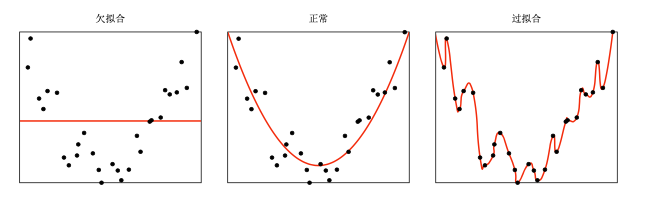
\includegraphics[width=1\textwidth]{figs/过(欠)拟合.png}
\caption{欠拟合和过拟合}
\label{欠拟合和过拟合}
\end{figure}

\subsubsection{ 结构风险：提高泛化能力}
%泛化问题：从训练数据到未见样本

机器学习中，模型的优化并不仅限于在训练集上的表现，更需要权衡模型在未见样本上的泛化能力。
机器学习的目标是在模型复杂度与泛化能力之间找到平衡，即找到一个能够在训练数据和未见样本上都表现良好的“理想模型”。

单纯最小化经验风险可能会导致过拟合，即模型过度拟合训练数据中的噪声，反而在未知数据上表现差。为了解决这一问题，机器学习引入了{\bf 结构风险最小化}（SRM, Structural Risk Minimization）作为对经验风险优化过程的扩展。

\begin{definition}[结构风险（Structural Risk）]
结构风险是指在考虑训练数据上经验风险的基础上，引入模型的复杂度约束，选择一个具有良好泛化能力的模型。其形式为：
\begin{equation}\label{eq:SRM}
R_{\rm SRM}(f) = R_{\rm emp}(f) +\lambda \Omega(f)
\end{equation}
其中，~$\Omega(f)$ 是正则化项，用于惩罚模型的复杂度，~$\lambda$ 是权衡经验风险与模型复杂度的超参数。最小化此目标函数的模型~$\hat{f}$ 则为理想模型。 
\end{definition}

{\bf 正则化}（Regularization）是机器学习中用于控制模型复杂度的一种技术。通过在损失函数中引入额外的约束项（即正则项），正则化能够避免模型过度拟合训练数据，提升其在未见数据上的泛化能力。

正则项通常用于对模型的复杂度进行惩罚，常见的正则化方法包括~$L_1$正则化（Lasso）和~$L_2$正则化（Ridge）。~$L_1$正则化（Lasso）通过在损失函数中加入模型参数的绝对值和，从而促使一些参数趋近于零，达到特征选择的效果，适用于希望得到稀疏模型的情况。~$L_2$正则化（Ridge）通过加入模型参数的平方和，惩罚大权重值，从而避免模型过于依赖某些特征，适用于希望保持所有特征但控制其权重的情况。

模型的复杂度通常指模型的自由度，即模型能够拟合训练数据的能力。复杂度过高时，模型可能过度拟合训练数据，捕捉到数据中的噪声，导致泛化能力差；而复杂度过低时，模型可能无法充分学习数据的规律，导致欠拟合。正则化项的引入有效地控制了模型的复杂度，确保其既不过拟合，也不欠拟合。

通过在优化目标中加入正则化项（如$ \Omega(f) $），结构风险最小化（SRM）能够平衡模型在训练数据上的拟合能力和在未知数据上的预测能力。具体而言，正则化项的大小通过超参数$\lambda$进行调节，$\lambda$越大，正则化的影响越强，模型的复杂度越低；$\lambda$越小，正则化的作用越弱，模型更加自由地拟合训练数据。

结构风险最小化是解决模型过拟合问题的关键策略之一，它通过引入正则化来对模型的复杂度进行惩罚，使得模型不仅在训练数据上表现良好，还能够有效地推广到未见的数据上，减少泛化误差。

%结构风险与经验风险的关系：
%经验风险侧重于优化训练集上的损失；
%结构风险则引入了一个正则化项来约束模型复杂度，避免在训练数据上过度拟合，从而提升模型的泛化能力。
%这种方法可以被看作是对“偏差-方差”权衡的另一种表达，结构风险最小化通过在优化经验风险时引入复杂度控制，降低了模型的方差，从而提高了泛化能力。

%\subsubsection{ 风险最小化与损失函数}
%损失函数作为模型优化的基础工具，在风险最小化中的作用可以分为以下几个层次：
%\begin{enumerate}
%\item[(1)] {\bf 刻画误差：}损失函数提供模型预测值与真实值之间误差的度量工具；
%\item[(2)] {\bf 经验风险：} 训练数据上损失函数的均值构成了经验风险，为模型的参数优化提供目标；
%\item[(3)] {\bf 期望风险：} 损失函数通过最小化经验风险来间接优化期望风险，找到在整个真实分布中表现良好的模型，实现更优的预测性能与泛化能力。
%\end{enumerate}

{\bf 机器学习的核心：从有限数据到一般规律}

机器学习的本质是从有限、高维、有噪声的数据中提取一般性规律的过程。给定一个训练集，机器学习的目标是从假设空间中找到一个泛化误差较低的“理想”模型，使其能够对未见的样本作出准确预测，尤其是那些不在训练集中出现的样本。
损失函数、经验风险与期望风险共同构成了这一过程的优化框架。通过合理设计损失函数并优化经验风险，机器学习模型不仅能够拟合训练数据，还能在未知样本上展现出优异的泛化能力。这种从数据到规律的转换正是机器学习成功的关键。

\subsection{优化：找到最优参数}

\subsubsection{参数与超参数}

在机器学习中，模型的参数分为参数和超参数。

优化又可以分为参数优化和超参数优化。模型~$f ({\bf x}; \theta)$ 中的~$\theta$ 称为模型的{\em 参数}（Parameters），是指模型在训练过程中通过学习得到的数值，通常是通过某种优化方法迭代调整得到的。
例如，在线性回归中，模型的权重和偏置就是参数；在神经网络中，每一层的权重矩阵和偏置项都是需要优化的参数。模型的参数是通过优化过程（如梯度下降）不断调整的，以最小化损失函数，从而让模型尽可能拟合训练数据，并具备较好的泛化能力。

除了可学习的参数~$\theta$之外，还有一类参数称作超参数(Hyper-parameters)。
超参数是模型训练之需要设定的参数，这些参数决定了模型的结构或优化策略。常见的超参数包括：聚类算法中的类别个数、梯度下降法的步长(学习率、)、正则项的系数、神经网络的层数、支持向量机中的核函数等。
超参数的选择对模型性能至关重要，合适的超参数能帮助模型快速收敛，避免陷入局部最小值或过拟合。而不合适的超参数则可能导致训练过程非常缓慢，甚至得不到一个有意义的解。
超参数并不直接参与模型的训练过程，而是通过试验和优化来调节模型的训练行为。

超参数的选择一般依赖于经验、交叉验证等技术来确定。在实践中，可以采用网格搜索、随机搜索或贝叶斯优化等方法来寻找最优的超参数组合。

在机器学习中，{\bf 优化}是一个调整模型参数使损失函数达到最小值的过程。
损失函数衡量的是模型的预测值与真实值之间的差距，优化的目标就是调整模型参数，使得这种差距尽可能小。优化不仅仅是减少训练数据上的误差，还要兼顾模型在未知数据上的表现，这就是我们所说的泛化能力。

优化过程的核心目标是通过最小化经验风险来逼近理想的期望风险，以此获得一个在整个数据分布中表现良好的模型。同时，优化过程中需要考虑结构风险，引入正则化来控制模型的复杂度，避免过拟合。通过优化，模型可以逐步调整参数，使其在训练集和未知数据集上都能取得较好的性能。

优化过程可以被视为在损失函数的搜索空间中寻找最优解的过程。这个过程通常依赖于梯度下降等算法，通过逐步调整模型参数，沿着梯度下降的方向逐步逼近最优解。

subsubsection{ 常见的优化方法}

优化算法的选择直接影响着训练过程的效率和结果。以下是几种常见的优化方法，它们各有特点，并在不同的任务和场景下发挥着不同的作用。 

% \subsubsection*{凸优化}
%为了充分利用凸优化中一些高效、成熟的优化方法，比如共轭梯度、拟牛 顿法等，很多机器学习方法都倾向于选择合适的模型和损失函数以构造一个凸 函数作为优化目标。但也有很多模型(比如神经网络)的优化目标是非凸的，只能退而求其次找到局部最优解。

 {\bf 梯度下降法（Gradient Descent）} 

在机器学习中，梯度下降法是最简单、最常用的优化方法，其基本思想是通过计算损失函数关于模型参数的梯度（即导数），沿着梯度的反方向更新参数，使损失函数的值逐渐减少，从而减少模型误差。
\begin{equation}\label{eq:gd}
    \theta_{t+1} = \theta_t - \eta \cdot \nabla_\theta L =   \theta_t - \eta \cdot \frac{\partial \mathcal{R_D}(\theta)}{\partial \theta}    
\end{equation}
    其中~$ \theta_t$是第~$t$次迭代时的参数值，~$\eta$ 是学习率(learning rate），决定参数更新的步长。
    
梯度下降法的关键在于每次参数更新时如何选择学习率，学习率决定了每次更新步长的大小。选择合适的学习率可以加速收敛，但学习率过大会导致跳跃过最优解，过小则会导致收敛过慢。
   
%梯度下降的变种包括：
%\begin{itemize}
%\item  {\bf 批量梯度下降（Batch Gradient Descent）： }每次迭代时，批量梯度下降需要计算每个样本上损失函数的梯度并求和，使用整个训练集来计算梯度，从而得到一个全局的更新方向。这种方法计算稳定，但在大数据集上计算开销较大，收敛速度较慢。
%\item  {\bf 随机梯度下降（（Stochastic Gradient Descent, SGD）:}  与批量梯度下降不同，SGD每次更新参数时只采集一个样本来计算梯度，这样每次参数更新非常迅速，计算开销较小。当经过足够次数的迭代时，随机梯度 下降也可以收敛到局部最优解[Nemirovski et al., 2009]。尽管SGD的收敛速度较快，但它的更新方向波动较大，收敛过程可能不稳定，甚至在某些情况下会错过最优解。随机梯度下降适用于大规模数据集。
%\item  {\bf 小批量梯度下降（Mini-batch Gradient Descent）：} 小批量梯度下降结合了批量梯度下降和SGD的优点，每次更新时使用一个小批量的数据进行计算。小批量梯度下降既能提高计算效率，又能保持梯度更新的稳定性，通常是现代深度学习中最常用的优化方法。
%\end{itemize}
 
 \begin{itemize} 
\item  {\bf 批量梯度下降（Batch Gradient Descent）： }每次迭代时，批量梯度下降需要计算每个样本上损失函数的梯度并求和，使用整个训练集来计算梯度，从而得到一个全局的更新方向。这种方法计算稳定，但在大数据集上计算开销较大，收敛速度较慢。
 \item {\bf 随机梯度下降（（Stochastic Gradient Descent,）:}  与批量梯度下降不同，随机梯度下降每次更新参数时只采集一个样本来计算梯度，这样每次参数更新非常迅速，计算开销较小。当经过足够次数的迭代时，随机梯度 下降也可以收敛到局部最优解[Nemirovski et al., 2009]。尽管随机梯度下降的收敛速度较快，但它的更新方向波动较大，收敛过程可能不稳定，甚至在某些情况下会错过最优解。随机梯度下降适用于大规模数据集。
 \item {\bf 小批量梯度下降（Mini-batch Gradient Descent）：} 小批量梯度下降结合了批量梯度下降和随机梯度下降的优点，每次更新时使用一个小批量的数据进行计算。小批量梯度下降既能提高计算效率，又能保持梯度更新的稳定性，通常是现代深度学习中最常用的优化方法。
\end{itemize}

在机器学习中，我们假设每个样本都是独立同分布的从真实数据分布中随机抽取出来的，真正的优化目标是期望风险最小。批量梯度下降相当于是从真 实数据分布中采集 N 个样本，并由它们计算出来的经验风险的梯度来近似期 望风险的梯度。为了减少每次迭代的计算复杂度，我们也可以在每次迭代时只 采集一个样本，计算这个样本损失函数的梯度并更新参数，即随机梯度下降法。

{\bf 动量法（Momentum）}动量法通过引入一个“惯性”项，即将之前几次梯度的加权平均与当前梯度结合，来调整参数更新的方向和步长。动量法能加速收敛，特别是在优化过程中遇到平坦区域时。通过这种方法，参数在更新时会带有一定的历史梯度“惯性”，从而减少了震荡现象，提升了收敛效率。
 
{\bf 自适应学习率方法}
 
自适应学习率方法根据训练过程中的梯度历史信息动态调整每个参数的学习率，可以加速收敛并提高稳定性。这类方法通过自动调整学习率，使得每个参数都能够根据其重要性得到合适的学习率。

常见的自适应学习率方法包括 
 \begin{itemize} 
\item AdaGrad （Adaptive Gradient Algorithm）根据参数的历史梯度的平方和，动态调整每个参数的学习率。 对于经常更新的参数，学习率会变小；对于很少更新的参数，学习率则相对较大。这样可以有效处理稀疏数据，尤其适用于文本数据和推荐系统。
AdaGrad能够很好地处理稀疏数据，自动调整每个参数的学习率，减少人为设定学习率的难度。但是，随着训练过程的进行，AdaGrad的学习率会逐渐衰减，可能导致后期学习率过小，导致收敛停滞。

\item RMSProp（Root Mean Square Propagation）是AdaGrad的一种改进方法，解决了AdaGrad中学习率衰减过快的问题。RMSProp使用梯度的指数加权移动平均来修正梯度的平方值，避免了学习率过早衰减的问题。
RMSProp有效缓解了AdaGrad的学习率衰减问题，能够更稳定地进行训练，适用于处理深度神经网络等复杂模型。
然而，这个方法需要调整一个衰减因子来控制历史梯度的影响，但一般而言，RMSProp在大多数任务中表现良好。

\item Adam（Adaptive Moment Estimation）结合了动量法和RMSProp的优点，既考虑了梯度的均值（动量）又考虑了梯度的方差（RMSProp）。Adam通过计算梯度的一阶矩（均值）和二阶矩（方差）的估计来调整学习率，使得每个参数的更新更为精准，收敛速度更快。  Adam的收敛速度快，广泛应用于大多数深度学习任务，能够有效应对稀疏梯度和不稳定的目标函数，但有时可能需要手动调整部分超参数，如学习率和衰减率。 
\end{itemize}
  
 \subsubsection*{牛顿法与共轭梯度法（Newton's Method and Conjugate Gradient）} 这些优化方法通过使用二阶导数（Hessian矩阵）来计算梯度，能够更加精准地确定参数的更新方向。它们的收敛速度较快，但计算开销较大，特别是在处理高维数据时。共轭梯度法是一种用于求解大型线性系统的高效方法，适用于二次优化问题。  

优化过程虽然是一个寻找最优解的过程，但仍面临不少挑战。优化方法的选择与超参数的设定对最终的训练效果有着重要的影响。以下是几个常见的优化挑战：
 \begin{itemize} 
\item 局部最小值与鞍点：机器学习中的损失函数通常是非凸的，存在多个局部最小值和鞍点。梯度下降等优化方法可能会在局部最小值或鞍点处停滞，导致无法找到全局最优解。为解决这一问题，通常会使用多次初始化策略，即从不同的随机起点开始优化，来避免陷入局部最小值。
\item 学习率的选择：学习率是优化算法的一个重要超参数，控制了每次参数更新的步长。过大的学习率可能会导致优化过程不稳定，甚至跳过最优解；而过小的学习率则可能使得优化过程过于缓慢，浪费时间。选择一个合适的学习率可以加速收敛过程，因此学习率调整技巧（如自适应学习率）成为现代优化算法中的常见设计。
\item  过拟合与欠拟合：在训练过程中，过拟合和欠拟合是常见的风险。过拟合通常发生在模型过于复杂时，导致它在训练数据上表现良好，但在未知数据上表现差；而欠拟合则是模型过于简单，无法有效地拟合训练数据。这两种现象都影响模型的泛化能力，因此在优化过程中必须加以注意。
  \end{itemize}

优化不仅仅是理论问题，它在实际应用中发挥着重要作用。无论是深度学习、支持向量机、强化学习，还是其他机器学习领域，优化算法都在确保模型训练效果和提升性能方面起着至关重要的作用。在实际应用中，优化的效果也往往决定了模型能否在现实世界中有效运作。例如，在自然语言处理任务中，优化算法能决定语言模型的表现，而在计算机视觉任务中，优化方法的选择则直接影响图像识别精度。

 \subsection{机器学习三要素的协同作用}
在机器学习的框架中，模型、损失函数和优化方法是三大核心要素，它们共同决定了模型的学习过程和最终的性能。
{\bf 模型}提供了解决问题的结构，是数据输入与预测输出之间映射关系的表达。
{\bf 损失函数}定义了优化的目标，用于衡量模型在任务中的表现。
{\bf 优化方法}则是寻找最优解的手段，帮助模型在候选空间中找到最优解。

机器学习任务的起点是明确输入空间与输出空间的定义。接下来，选择一个合适的模型来近似真实的映射函数~$f(x)$ 或真实条件概率分布~$P(y|x)$。

不同的机器学习任务通常会在输入空间与输出空间上有所区别，同时根据任务的需求选择适合的模型。
线性模型和非线性模型的核心差异在于函数~$ f(x, \theta)$的表示形式不同。统计方法和非统计方法则在学习准则上有所不同， 如	期望风险、经验风险、结构风险等概念的使用。

机器学习算法的差异，通常体现在模型结构、损失函数和优化方法的不同。
相同的模型结构可以通过不同的损失函数和优化方法进行训练。例如，对于线性分类问题，虽然感知器、逻辑回归和支持向量机（SVM）都采用了线性模型，但它们在损失函数和优化策略上有所不同：感知器基于误分类点设计损失函数，逻辑回归使用对数似然损失，而支持向量机则通过最大化间隔来构建损失函数。

这三要素的协同作用贯穿机器学习的整个过程，从模型的设计到损失函数的构建，再到优化方法的选择，它们共同影响着模型学习的效果与效率。
通过不同模型结构、损失函数和优化策略的组合，机器学习展示了其强大的多样性与灵活性，也使其能够解决从简单回归问题到复杂图像识别任务的各种应用。

机器学习的成功，依赖于模型、损失函数和优化方法的紧密结合。模型定义了任务的表达形式，损失函数为学习提供了明确的目标，而优化方法则是最小化损失函数的工具。在实际应用中，合理的模型选择、合适的损失函数设计和高效的优化方法，是构建高效机器学习系统的关键。

 \section{传统机器学习}
% \section{主要的机器学习范式}

%机器学习的不同范式依据数据的标注情况、学习目标和反馈方式进行区分。常见的机器学习范式包括监督学习、半监督学习、无监督学习和强化学习。每种范式在问题建模、数据处理和学习方法上具有独特的特点和应用场景。

机器学习的任务可以根据训练样本提供的信息和反馈方式的不同，划分为三种主要的学习范式：{\bf 监督学习}、{\bf 无监督学习}和{\bf 强化学习}。这三种方式的核心区别在于输入数据是否标注、模型训练过程中是否提供明确的目标信号以及反馈机制的设计。

\subsection{ 监督学习 (Supervised Learning)：通过标注数据进行映射学习}

%用数据挖掘领域大家韩家炜教授的观点\cite{han2011data}来说，
%所有的监督学习（Supervised Learning），基本上都是“分类（Classification）”的代名词。

监督学习从有标签的训练数据中学习模型，然后给定某个新数据，利用模型预测它的标签。这里的标签，其实就是某个事物的分类。

比如，小时候父母告诉我们某个动物是猫、是狗或是猪，然后在我们的大脑里就会形成或猫或狗或猪的印象（相当于模型构建），然后面前来了一条“新”小狗，如果你能叫出来“这是一只小狗”，那么恭喜你，标签分类成功！但如果你回答说“这是一头小猪”。这时你的监护人就会纠正你的偏差，“乖，不对，这是一只小狗”，这样一来二去地进行训练，不断更新你大脑的认知体系，聪明如你，下次再遇到这类新的“猫、狗、猪”等，你就会天才般地给出正确的“预测”分类（示意图如图3-1所示）。

事实上，整个机器学习的过程就是在干一件事，即通过训练，学习得到某个模型，然后期望这个模型也能很好地适用于“新样本”（即预测）。这种模型适用于新样本的能力，也称为“泛化能力”，它是机器学习算法非常重要的性质。

在学习过程中，需要使用训练数据，而训练数据往往是人工给出的。在这个训练集合中，系统的预期输出（即标签信息）已经给出，如果模型的实际输出与预期不符（二者有差距），那么预期输出就有责任“监督”学习系统，重新调整模型参数，直至二者的误差在可容忍的范围之内。因此，预期输出（标签信息）也被称为“教师信号”。

监督学习是最常见的机器学习范式，主要应用于标注数据充足的场景。在监督学习中，训练数据集由输入-输出对（即特征和标签）组成，学习的目标是通过训练模型来预测输入数据对应的标签。监督学习的核心任务是通过最小化损失函数，使模型能够从标注数据中学习到输入与输出之间的映射关系。

监督学习需要提供大量标注好的训练样本。每个样本由输入（$X$）和期望输出（$Y$）组成，模型通过学习从输入到输出的映射函数$f: X \rightarrow Y$，使得模型预测的输出尽可能接近真实标签，从而最小化预测输出与真实标签之间的误差。

根据标签类型的不同，监督学习可以进一步分为分类（Classification）和回归（Regression）两种任务，分别对应离散和连续标签的预测需求。

{\bf  1. 分类（Classification）}

分类问题的目标是将输入数据划分到不同的类别中，输出为离散的类别标签，标签取值离散且有限（如 0/1、类别 A/B/C 等）。分类问题的训练目标是最大化样本分配到正确类别的概率。分类问题的常用算法包括逻辑回归、支持向量机（SVM）、决策树、随机森林、神经网络等。

分类问题的典型应用包括：
\begin{itemize}
\item {\bf 手写数字识别：}输入是手写数字的图像，输出是数字标签（如 0-9）。
 \item {\bf  垃圾邮件检测：}输入是邮件文本内容，输出是类别标签（垃圾邮件或非垃圾邮件）。
\item {\bf  图像分类：}输入是一张图片，输出是图像所属的类别标签（如猫/狗）。
\end{itemize}

 {\bf  2. 回归（Regression）}
 
 回归问题的目标是根据输入特征预测一个连续的数值结果，标签取值是实数或连续整数（如温度、房价）。
回归问题的常用算法包括线性回归、岭回归、LASSO 回归、决策树回归、神经网络等。

回归问题的典型应用包括：
\begin{itemize}
 \item {\bf 房价预测：}输入是房屋的特征（如面积、房间数、位置），输出是房价的具体数值。
\item {\bf  工资预测：} 输入是员工的相关特征（如年龄、教育背景、工作年限），输出是对应的工资。
 \item {\bf 股票价格预测：}输入是历史股价和其他影响因素，输出是未来的股价。
\end{itemize}

%{\bf  对比分类与回归}
%
%| 类别         | 标签类型           | 任务目标                  | 典型任务               | 常用指标       |
%|-------------------|------------------------|-------------------------------|----------------------------|--------------------|
%| 分类         | 离散值                | 输出样本所属类别              | 手写数字识别、垃圾邮件检测 | 准确率、F1 分数    |
%| 回归         | 连续值                | 预测目标值的具体数值          | 房价预测、工资预测         | 均方误差、绝对误差 |
%根据问题的特点选择合适的任务类型，可以更高效地构建模型并解决实际问题。  

监督学习
- {\bf 数据需求：}
  - {\bf 输入}：标注好的样本对 $(X, Y)$，
  - {\bf 反馈}：明确的错误信号（如预测值和真实值的差距）。
  
- {\bf 特点}：
  - 数据标注成本高，尤其在图像分类、语音识别等需要人工标注的任务中。
  - 适合有明确目标的任务，例如分类、回归和生成任务。

监督学习需要标注好的数据样本对 $(X, Y)$，如图像与其对应的分类标签，文本与其翻译结果。训练时，模型通过最小化预测值与真实值的差距来优化。监督学习的典型算法包括线性回归、逻辑回归、支持向量机（SVM）、决策树、随机森林和神经网络等。
监督学习适用于有明确目标的任务，广泛应用于图像分类、语音识别、机器翻译等领域，但数据标注成本较高。

\subsubsection{支持向量机：几何之美，划分世界 还是优雅地划分世界}
在深度学习成为 AI 主角之前，支持向量机（（Support Vector Machine, SVM）曾是机器学习的“扛把子”。它以简洁的数学结构、优雅的几何思想和强大的泛化能力，它以简洁、强大、可解释的特性，长期在分类任务中独领风骚，尤其在样本数量不多但维度较高的情况下，表现十分优越。

即便在今天，SVM 仍然是理解“什么是机器学习”的一把钥匙。它告诉我们：{\bf 学习，不是把所有点都记住，而是找到一条分得最稳妥的界线。}

\subsection{支持向量机的基本思想：最大间隔与支持向量}
%最大间隔 和支持向量，是支持向量机的基本思想。

支持向量机（SVM）是一种监督学习算法，用于解决分类问题（也可扩展到回归）。它的核心思想是：在特征空间中，寻找一条能够“最大限度地区分”不同类别样本的决策边界。
SVM 不仅要求分类正确，还要求分得最稳：距离边界最近的样本点越远，模型越具有泛化能力。

想象平面上有两类数据点，红点和蓝点。你想找到一条直线把它们分开。如图~\ref{2class}所示，很多线都可以把两类点分开，但哪条最好？
\begin{figure}[htbp]
\centering
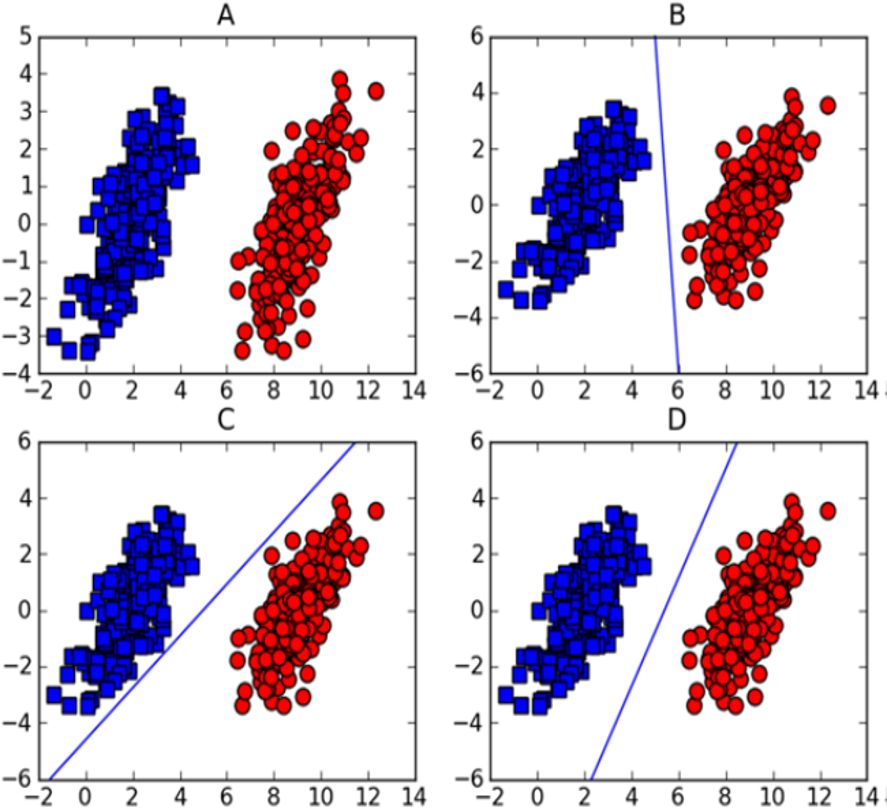
\includegraphics[width=0.6\textwidth]{figs/2class.png}
\caption{哪条线分隔得更好？}
\label{2class}
\end{figure}
%（二维平面中的直线，三维空间中的平面，更高维空间中超平面），能将这两类点尽可能“干净利落”地分开。

很多分类算法都试图寻找这样的边界，但支持向量机（SVM）的哲学则更进一步：不仅要“分开”，更要“分得稳”。SVM关注的不仅是“能否区分”，而是“在最难区分的样本面前，也能留出足够的余地”。

SVM的目标是寻找一个既能正确分类，又能与两类样本中离边界最近的那些点保持最大距离的超平面，也就是具有最大间隔（Margin）的分界线。因为，这种分界线更加“稳健”，不会因为数据的微小扰动就改变分类结果。

那些恰好位于边界附近、起到“支撑作用”的样本点，被称为{\bf 支持向量（Support Vectors）}。
支持向量决定了分类边界的位置，其余样本点对模型结果的影响微乎其微。
换句话说，SVM 并不是关注所有样本，而是聚焦于那一小部分最“危险”的边缘点——即最接近分类边界、最容易被误判的样本。

SVM要确保，哪怕面对这些最难处理的样本，也仍然能够稳妥地区分开来。通过最大化两类样本之间的间隔，找出离两类最近样本仍然有最大余地的那条超平面，从而构造出最具鲁棒性的决策边界。

这种“最大间隔”的策略，不仅提供了清晰的几何直觉，还带来了两个显著优势：
\begin{enumerate}
    \item \textbf{更强的泛化能力}：更大的间隔意味着决策边界更稳健，对未见过的新样本表现更好；
    \item \textbf{更少的模型依赖}：模型的边界仅由支持向量决定，训练数据中的大部分样本几乎不影响最终的分类器，这让 SVM 在模型复杂度控制方面具有天然优势。
\end{enumerate}

正是这种“只关心最难分样本”的策略，使得 SVM 并不是从全局平均中得出一个“中庸”的结论，而是专注于在关键点上做出最稳妥的判断。这也为后续引入核函数、处理非线性分类问题打下了坚实的基础——无论在何种维度中，SVM 始终遵循一条核心准则：\emph{找到间隔最大的决策边界，仅由“支持向量”决定其位置}。

最大间隔，最小依赖，这正是支持向量机“少即是多”的优雅体现。

%\begin{figure}[htbp]
%\centering
%\includegraphics[width=1\textwidth]{figs/支持向量机的最大间隔思想.png}
%\caption{支持向量机的最大间隔思想（图源：Wikipedia）}
%\label{支持向量机的最大间隔思想}
%\end{figure}

\subsubsection{线性可分情形：最大间隔的几何理解}

考虑最简单的情况：输入样本数据在原始特征空间是线性可分的。也就是说，存在一个线性分类边界能够完全正确地区分两类样本。

我们希望不仅仅找到一个“能够分开”的“决策边界”，更要找到一个“分得最稳”的边界，也就是一个能在两类样本之间留出最大间隔（margin）的超平面。
% 将两类样本完全正确地区分开来，并且它们之间存在一个“安全间隔”，没有任何样本落入这个间隔带内。

假设我们有如下的训练数据：
\[
\{({\bf x}_1, y_1), ({\bf x}_2, y_2), \dots, ({\bf x}_n, y_n)\}, \quad {\bf x}_i \in \mathbb{R}^d, \quad y_i \in \{+1, -1\}
\]
其中，${\bf x}_i$ 是样本特征向量，$y_i\in \{+1, -1\}$ 是类别标签，分别对应正类和负类。

我们希望学习一个能在两类样本之间留出最大间隔（margin）的超平面，即线性平面
\begin{equation}\label{hyper_plane}
{\bf w}^T {\bf x} + b  = 0
\end{equation}
其中，${\bf w} \in \mathbb{R}^d$ 是法向量，决定超平面的方向；$b \in \mathbb{R}$ 是偏置项，决定超平面到原点的距离，~${\bf x}$是输入特征向量。

%也就是说，我们希望找到最优的参数~${\bf w}$ 和~$b$，使得对于每个样本~$({\bf x}_i,y_i)$，都满足
%$$
%y_i({\bf w}^T {\bf x}_i+b)\ge 1
%$$
%这就确保正类~$y_i=+1$ 在~${\bf w}^T {\bf x} + b  \ge 1$一侧，而负类~$y_i-1$ 在~${\bf w}^T {\bf x} + b  \le -1$ 一侧， 而两类之间留出了“安全间隔”带。 

%\subsubsection{函数间隔与几何间隔的区别与联系}

在理解支持向量机的最大间隔原理之前，我们需要先区分两个相关但含义不同的概念：函数间隔（Functional Margin）与几何间隔（Geometric Margin）。

\paragraph*{函数间隔---基于内积，体现分类置信度}

函数间隔来源于早期的感知机模型，其本质是一个基于超平面内积的数值，用于衡量某个样本点被当前超平面分类的分类置信度---多“自信”。样本点~${\bf x}_i$ 的函数间隔被定义为
\begin{equation}\label{eq:func_margin}
\gamma_i^{\text{func}} = y_i({\bf w}^T {\bf x}_i + b )
\end{equation}
其中，$y_i \in \{+1, -1\}$ 是样本~${\bf x}_i$的类别标签，${\bf w}$ 是超平面法向量，$b$ 是偏置项。函数间隔表示模型对样本分类的“置信度”，但它本身并不具备“距离”的几何意义，因为它会随着 ${\bf w}$ 的缩放而变化，因而仅表示该样本点被正确分类的相对置信度。

\paragraph*{ 几何间隔---点到超平面的真实距离}
%我们真正关心的是样本 ${\bf x}_i$ 到超平面 ${\bf w}^T {\bf x} + b  = 0$ 的\textbf{几何间隔（geometric margin）}，即“垂直距离”。
几何间隔考虑的是一个样本点到超平面的“垂直距离”，即几何意义上的最短距离。
根据解析几何，样本点 ${\bf x}_i$ 到超平面 ${\bf w}^T {\bf x} + b  = 0$ 的垂直距离为
\begin{equation}\label{eq:geom_margin}
\gamma_i^{\rm geo} = \frac{y_i({\bf w}^T {\bf x}_i + b )}{\|{\bf w}\|}. %=\frac{\gamma_{\rm fun}}{\|{\bf w}\|}.
\end{equation}

函数间隔反映模型对当前样本的分类置信度，而几何间隔则给出了样本与决策边界的实际距离。
可以看出，函数间隔~\eqref{eq:func_margin}与几何间隔~\eqref{eq:geom_margin}之间仅差一个比例因子$\|{\bf w}\|$：
\[
\gamma_i^{\text{geo}} = \frac{\gamma_i^{\text{func}}}{\|{\bf w}\|}
\]
也就是说，几何间隔是函数间隔除以超平面法向量的模长。几何间隔对 $b$ 进行了归一化，因此它具有明确的度量意义，不受超平面缩放的影响。

注意到，参数~$({\bf w},b)$ 和参数~$(k{\bf w},kb)$表示相同的超平面~\eqref{hyper_plane}。这意味着， 在不改变决策边界位置的前提下，我们可以“自由地缩放”参数 ${\bf w}$ 和 $b$。不失一般性，我们可以人为规定支持向量满足
$$
y_i({\bf w}^T {\bf x}_i + b) = 1
$$
这就是所谓的归一化函数间隔。

为了令分类结果具有更强的鲁棒性，SVM确保分类正确并留出“安全边界”---样本距离超平面“足够远”。因此，所有训练样本满足如下约束：
\begin{equation*}
y_i ({\bf w}^T {\bf x}_i + b+ b ) \geq 1, \quad \forall i = 1, \dots, n.
\end{equation*}
这等价于
\begin{equation}\label{eq:SVM}
\begin{cases}
\mbox{ 对于正类样本 }\, (y_i = +1) \mbox{，要求 } \; {\bf w}^T {\bf x}_i + b  \geq +1;\\
\mbox{ 对于负类样本}\; (y_i = -1)\mbox{ ，要求 }\; {\bf w}^T {\bf x}_i + b  \leq -1;
\end{cases}
\end{equation}
换句话说，正类样本位于超平面 ${\bf w}^T {\bf x} + b  = 1$ 一侧，负类样本则位于 ${\bf w}^T {\bf x} + b  = -1$ 一侧，且都距离超平面各有 1 个单位的“间隔带”，从而两个超平面之间夹着一个宽度为  $\frac{2}{\|{\bf w}\|}$ 的间隔带。%不允许任何训练样本落入其中。
这个区间就是我们想要最大化的“间隔”。

%\begin{center}
%\begin{tabular}{|c|c|c|c|}
%\hline
%\textbf{名称} & \textbf{表达式} & \textbf{来源} & \textbf{含义} \\
%\hline
%函数间隔 & $y_i({\bf w}^T {\bf x}_i + b )$ & 感知机模型 / 内积判别 & 分类置信度（未归一化） \\
%\hline
%几何间隔 & $\dfrac{y_i({\bf w}^T {\bf x}_i + b )}{\|{\bf w}\|}$ & 解析几何 & 到超平面的实际距离 \\
%\hline
%\end{tabular}
%\end{center}

在这个前提下，最大化几何间隔 $\text{Margin} = \frac{2}{\|{\bf w}\|}$ 的问题等价于最小化 $\|{\bf w}\|$。

由于$\|{\bf w}\| = \sqrt{{\bf w}^T {\bf w}}$ 是一个带有平方根的函数，在原点处不可导，从而在计算梯度、构造对偶问题、使用拉格朗日乘子法时，不易求解。因此，我们转而最小化与~$\|{\bf w}\|$ 有相同单调性且可导的光滑函数~$ \|{\bf w}\|^2 ={\bf w}^T {\bf w}$，以方便求梯度和使用最优化算法。此外，增加常数$\frac{1}{2}$作为缩放因子不影响最优解的位置，却在计算导数时让表达式更简洁：
$$
\frac{d }{d {\bf w}}\left(\frac{1}{2}{\bf w}^T {\bf w} \right) = {\bf w}
$$
这比直接对 ${\bf w}^T {\bf w}$ 求导结果更“干净”。

因此，求参数~${\bf w},b$使得超平面~${\bf w}^T+b=0$具有最近距离样本点最大间隔的问题，最终转化为如下优化问题
\begin{equation}\label{eq:SVM_opt}
\begin{aligned}
\min_{{\bf w},b} \quad & \frac{1}{2} \|{\bf w}\|^2 \\
\text{s.t.} \quad & y_i({\bf w}^T {\bf x}_i + b ) \geq 1 \quad i=1,\dots,n.
\end{aligned}
\end{equation}

这个优化问题中，目标是使分类间隔最大，即最小化 $ |w|^2 $；约束是所有样本都要被正确分类，且有至少 1 的“函数间隔”。
特别地，满足约束等号的样本（即 $y_i({\bf w}^T {\bf x}_i + b) = 1$）即为\textbf{支持向量（Support Vectors）}。它们正好落在间隔边界 ${\bf w}^T {\bf x} + b= \pm 1$ 上，决定了最终分类超平面的位置。其他远离边界的样本对模型无影响。

\eqref{eq:SVM_opt}的目标函数是凸函数，约束是线性的，因此整个问题是一个凸(二次)优化问题，这个问题不仅具有清晰的几何意义，也具有优良的数学性质---具有唯一的全局最优解，可通过拉格朗日对偶理论来求解。

\textbf{Step 1: 构造拉格朗日函数}

我们为每一个约束 $y_i({\bf w}^T  {\bf x}_i + b ) \geq 1$ 引入拉格朗日乘子 $\alpha_i \geq 0$，构造拉格朗日函数：
$$
\mathcal{L}({\bf w}, b,\alpha) =  \frac{1}{2} \|{\bf w}\|^2 -\sum_{i=1}^n \alpha_i \left(  y_i \left( {\bf w}^T {\bf x}_i +b\right)-1\right)
$$

我们使用对偶性原理：对 $w$ 和 $b$ 做极小，对 $\alpha$ 做极大，换句话说：
$$
{\rm max}_{\alpha >0} {\rm min}_{{\bf w}, b}\, \mathcal{L}({\bf w}, b, \alpha)
$$
我们先对 $w$ 和 $b$ 求偏导，使 $\mathcal{L}$ 极小。

\textbf{Step 2: 求对偶问题（Dual Problem）}

对 $\mathcal{L}$ 关于 ${\bf w}$ 和 $b$ 求偏导，并令其为零，得到最优条件：
$$
\frac{\partial\mathcal{L}}{\partial {\bf w}}= {\bf w}- \sum_{i=1}^n \alpha_i y_i {\bf x}_i
= 0 \Longrightarrow {\bf w}= \sum_{i=1}^n \alpha_i y_i {\bf x}_i
$$
$$
\frac{\partial\mathcal{L}}{\partial b}=- \sum_{i=1}^n \alpha_i y_i  = 0 \Longrightarrow  \sum_{i=1}^n \alpha_i y_i =0
$$
将这些代入原始拉格朗日函数~$\mathcal{L}$ ，得到对偶的优化形式（仅关于 $\alpha$）:
\begin{equation}\label{eq:svm_opt}
\begin{array}{c}
{\rm max}_{\alpha} \sum_{i=1}^n \alpha_i -\frac{1}{2} \sum_{i,j=1}^n \alpha_i \alpha_j y_i y_j {\bf x}_i^T {\bf x}_j \\
{\rm s.t.} \; \alpha_i \ge 0, \forall i=1, \dots, n \\
  \sum_{i=1}^n \alpha_i y_i =0
  \end{array}{c}
\end{equation}

\textbf{Step 3: 使用优化算法求解 $\alpha_i$}
\eqref{eq:svm_opt} 就是我们熟悉的支持向量机对偶优化问题，是一个标准的凸二次规划问题（Quadratic Programming, QP），可以用现成的优化器（如 cvxopt, quadprog, 或者 scikit-learn 中的 SVC）进行求解。得到最优解 $\alpha^\ast$ 后， 找到其中有非零 $\alpha_i$，即~$\alpha_i>0$，的样本点 ${\bf x}_i$ 就是 \textbf{支持向量}
可用于计算最终的参数~${\bf w}$ 和 $b$。 

\textbf{Step 4: 计算最终的超平面参数 ${\bf w}$ 和 $b$}
$$
{\bf w}= \sum_{i=1}^n \alpha_i y_i {\bf x}_i
$$
选择任意一个支持向量 ${\bf x}_s$（满足 $\alpha_s > 0$），可通过其计算 $b$：
$$
b= y_s -{\bf w}^T {\bf x}_s
$$
或者，为提高稳定性，可对所有支持向量求平均：
$$
b= \frac{1}{N_s} \sum_{s\in SV} \left( y_s - {\bf w}^T {\bf x}_s\right)
$$

\textbf{Step 5: 得到决策函数}

最终的决策函数为：
$$
f= {\rm sign}\left( y\, {\bf w}^T {\bf x} +b\right)= {\rm sign}\left(\sum_{i=1}^n \alpha_i y_i {\bf x}_i^T {\bf x} +b\right)
$$
%\begin{figure}[htbp]
%\centering
%\includegraphics[width=0.6\textwidth]{figs/linear_svm.png}
%\caption{线性可分支持向量机：最大间隔决策边界与支持向量}
%\label{fig:linear-svm}
%\end{figure}

以上就是支持向量机在线性可分情形下的基本原理：通过最大化间隔、聚焦关键样本，构建出鲁棒性更强、泛化能力更好的分类模型。
%如图~\ref{fig:linear-svm} 所示，
虽然大多数样本都被正确分类，但真正“支撑”决策边界的只有少数关键点——支持向量。

\subsubsection{简单示例：支持向量机的分类流程}~\label{sec:SVM_exs}

为了更直观地理解线性可分支持向量机的求解过程，
我们以一个二维数据集为例。假设我们有两个类别的点。

\begin{center}
\begin{tabular}{ccc}
\toprule
$x_1$ & $x_2$ & 类别 \\
\midrule
1 & 1 & A（+1） \\
2 & 2 & A（+1） \\
1 & 3 & A（+1） \\
5 & 6 & B（-1） \\
6 & 5 & B（-1） \\
7 & 7 & B（-1） \\
\bottomrule
\end{tabular}
\end{center}

\begin{figure}[htbp]
\centering
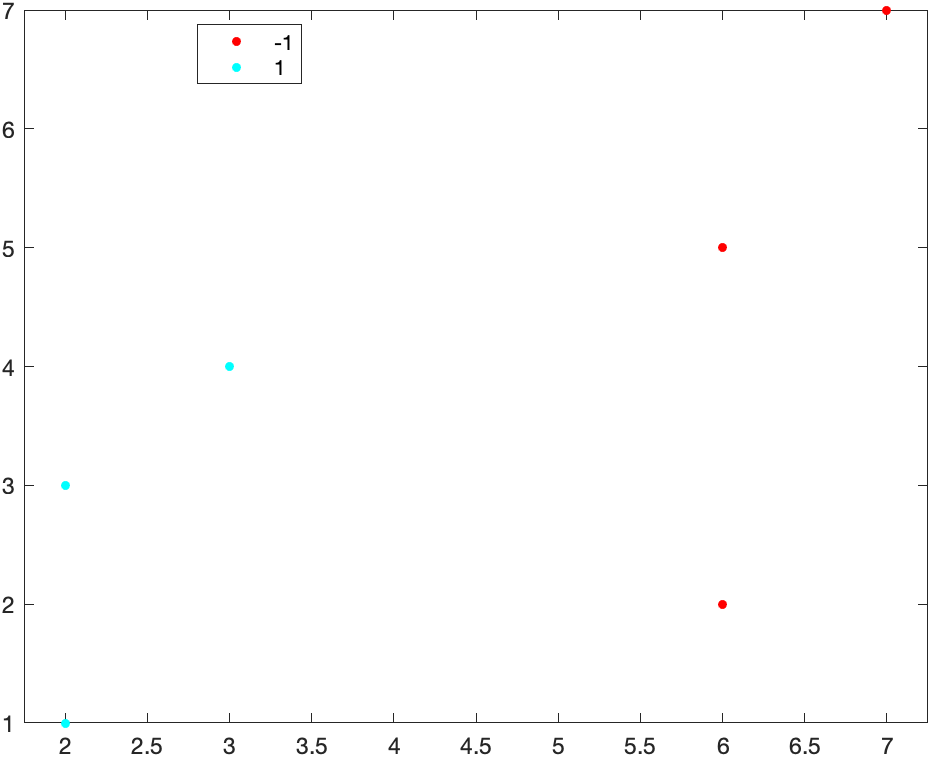
\includegraphics[width=0.6\textwidth]{figs/eg_hardSVM.png}
\caption{}
\label{eg_SVM}
\end{figure}

如图~\ref{eg_SVM}所示，这些点在二维平面上分布明显，可被一条直线良好划分。
我们的目标是使用 SVM 的方法，求出一个最大间隔的超平面（直线），实现对这两类样本的划分。

\vspace{0.5em}
\textbf{Step 1: 标注数据与变量定义}

设每个样本点为 ${\bf x}_i = [x_{i1}, x_{i2}]^T$，对应的类别标签为 $y_i \in \{+1, -1\}$。我们共有 6 个样本点，记为：
\[
\begin{aligned}
{\bf x}_1 = \left(
\begin{array}{c} 
1 \\ 
1 
\end{array}\right),\;  y_1 = +1;  & \quad {\bf x}_2 = \left(
\begin{array}{c} 
2 \\ 
2 
\end{array}\right), \;  y_2 = +1 ; & \quad{\bf x}_3 =  \left(
\begin{array}{c} 
1 \\ 
3 
\end{array}\right),\;  y_3 = +1 \\
{\bf x}_4 =  \left(
\begin{array}{c} 
6 \\ 
5 
\end{array}\right), \; y_4 = -1 ; &\quad {\bf x}_5 =  \left(
\begin{array}{c} 
5 \\ 
6 
\end{array}\right),\; y_5 = -1 ; &\quad {\bf x}_6 = \left(
\begin{array}{c} 
7 \\ 
7 
\end{array}\right),\; y_6 = -1 
\end{aligned}
\]

\vspace{0.5em}
\textbf{Step 2: 写出原始优化问题与对偶优化问题}

SVM 的优化目标是最小化：
\[
\min_{{\bf w}, b} \quad \frac{1}{2}\|{\bf w}\|^2
\quad \text{subject to:} \quad y_i({\bf w}^T {\bf x}_i + b) \geq 1,\quad \forall i = 1,\dots,6.
\]

记~$ \alpha_i $ 为第~$i$个样本的拉格朗日乘子，支持向量机的对偶优化问题为：
\begin{equation}\label{ex_opt}
\begin{array}{c}
{\rm max}_{\alpha} \sum_{i=1}^6 \alpha_i -\frac{1}{2} \sum_{i=1}^6 \sum_{j=1}^6 \alpha_i \alpha_j y_i y_j {\bf x}_i^T {\bf x}_j \\
{\rm s.t.} \;  \sum_{i=1}^6 \alpha_i y_i =0 \\
\alpha_i \ge 0, \forall i=1, \dots, 6 
   \end{array}
\end{equation}

\vspace{0.5em}
\textbf{Step 3: 计算内积矩阵（Gram 矩阵）}

计算出样本之间的点积~${\bf x}_i^T {\bf x}_j,i,j=1,\dots, 6$，构建出一个~$ 6\times 6$ 的Gram对称矩阵
\[
K =( \langle {\bf x}_i, {\bf x}_j \rangle)_{6\times 6} =
\left(
\begin{array}{cccccc} 
2 &  4  & 4 & 11  & 11   &14\\
4 &  8  & 8 & 22 & 22 &28 \\
4 &  8  & 10 & 23& 21&28 \\
11 &  22  &23  & 61& 60& 77 \\
11 & 22  &21 & 60& 61& 77 \\
14 & 28  & 28  &77 & 77 & 98 \\
\end{array} \right)
\]

于是，~\eqref{ex_opt} 变为如下形式
\begin{equation*}
\begin{array}{c}
{\rm max}_{\alpha} \sum_{i=1}^6 \alpha_i -\frac{1}{2} \sum_{i=1}^6 \sum_{j=1}^6 \alpha_i \alpha_j y_i y_j K_{ij} \\
{\rm s.t.} \; \alpha_i \ge 0, \forall i=1, \dots, 6 \\
  \sum_{i=1}^6 \alpha_i y_i =0
  \end{array}
\end{equation*}

可以用 QP（Quadratic Programming）求解器如 cvxopt 进行数值求解，得到最优解为
$$
 \alpha_1 =0,  \alpha_2 =0.0407(\mbox{正类}), \alpha_3 =0.0410(\mbox{正类}) , \alpha_4 =0.0816(\mbox{负类}), \alpha_5 =0, \alpha_6 =0 
$$
因此，样本~$x_2,x_3,x_4$ 为支持向量。

\vspace{0.5em}
\textbf{Step 4: 计算~${\bf w},b$}

通过优化计算，得到
$$
{\bf w}= \sum_{i=1}^6 \alpha_i y_i {\bf x}_i = 0.0407\cdot (+1) \cdot {\bf x}_2 +0.0410\cdot (+1) \cdot {\bf x}_3+0.0816\cdot (-1) \cdot {\bf x}_4 = \left(\begin{array}{c} -0.2859 \\ -0.2856\end{array}\right)
$$
选择任一支持向量求~$b$，如~$x_2 = \left( 2,2\right)^T, y_2= +1$ 得
$$
b= y_2 -{\bf w}^T x_2 = 1-(-0.2856\cdot 2 +(-0.2856)\cdot 2) =2.1428
$$

\vspace{0.5em}
\textbf{Step 5: 写出分类函数}

最终，分类决策函数为
\[
f(x) = \text{sign} \left( {\bf w}^T {\bf x}+b \right)= \text{sign}\left(-0.2859x_1 -0.2856 x_2 +2.1428\right)
\]
这就是分类边界。也就是说,
\begin{itemize}
\item 若 $-0.2859x_1 -0.2856 x_2 +2.1428 > 0$，判为 A 类（+1）；
\item 若 $-0.2859x_1 -0.2856 x_2 +2.1428 <  0$，判为 B 类（-1）。
\end{itemize}

%\vspace{0.5em}
%\textbf{Step 3: 观察并选取支持向量（假设）}
%
%从图上可以直观看出，点 $(3, 3)$ 和 $(6, 3)$ 位于边界附近，它们分别是正类和负类中距离分界线最近的点，因此我们假设这两个点为支持向量，并尝试构造满足以下约束的超平面：
%\begin{equation}\label{linear_eq}
%w^T[3,3]^T + b = +1 \\
%w^T[6,3]^T + b = -1
%\end{equation}
%
%将上式两式相减，得到：
%\[
%w^T([3,3] - [6,3]) = 2 \Rightarrow w^T[-4, 0]^T = 2 \Rightarrow -3w_1 = 2 \Rightarrow w_1 = -\frac{2}{3}
%\]
%
%代入方程组~\ref{linear_eq}的~$3w_2 +b = 1$，可求 $w_2$ 和 $b$的无穷多组解。 
%因此可以选择 $w_1 = -\frac{2}{3}$，$w_2 = 1$，$b = 0$ 为一个解（不唯一）。
%
%支持向量是距离分隔线最近的样本点。它们“支撑”着这个边界不倒，满足：
%\[
%y_i ({\bf w}^T {\bf x}_i + b ) \geq \pm 1, \quad \forall i=1，\dots, n
%\]
%这几个点对超平面的位置至关重要，其他点怎么动，边界都不动摇。
%  


\vspace{0.5em}
\textbf{Step 6: 新样本分类测试}

例如，
\begin{itemize}
\item 输入 $x = \left(
\begin{array}{c} 
3 \\ 
3 
\end{array}\right)$，
计算得 $f(x) = -0.2859 \cdot 3-0.2856 \cdot 3  +2.1428 =0.4283>0 $，则判为 A 类;
\item 输入 $x =\left(\begin{array}{c} 4 \\ 4\end{array}\right)$，计算得 $f(x) =-0.2859 \cdot 4 -0.2856 \cdot 4  +2.1428 =-0.1432  <0 $，则判为 B   类。
\end{itemize}

\begin{figure}[htbp]
\centering
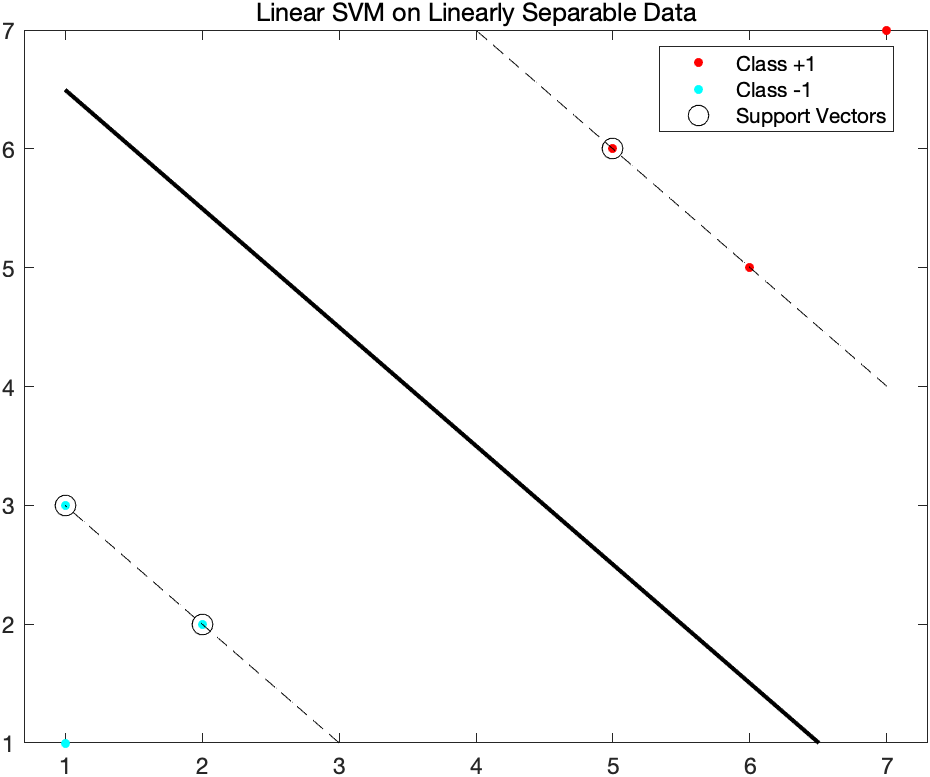
\includegraphics[width=0.72\textwidth]{figs/eg_hardSVM-plot.png}
\caption{}
\label{eg1_softSVM-plot}
\end{figure}

%\subsection{简单示例二：支持向量机的分类流程}
%
%为了更直观地理解线性可分支持向量机的求解过程，
%我们以一个二维数据集为例。假设我们有两个类别的点。
%
%\begin{center}
%\begin{tabular}{ccc}
%\toprule
%$x_1$ & $x_2$ & 类别 \\
%\midrule
%2 & 3 & A（+1） \\
%3 & 3 & A（+1） \\
%2 & 1 & A（+1） \\
%6 & 5 & B（-1） \\
%7 & 6 & B（-1） \\
%6 & 3 & B（-1） \\
%\bottomrule
%\end{tabular}
%\end{center}
%
%\begin{figure}[htbp]
%\centering
%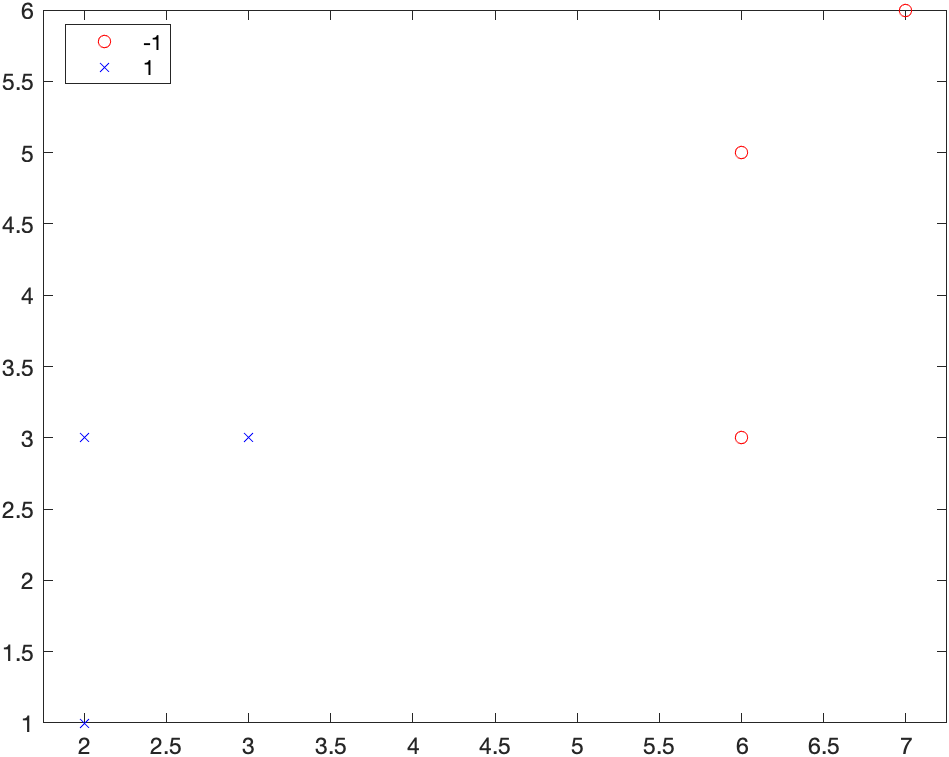
\includegraphics[width=0.6\textwidth]{figs/eg_softSVM.png}
%\caption{}
%\label{eg_softSVM}
%\end{figure}
%
%如图~\ref{eg_softSVM}所示，这些点在二维平面上分布明显，可被一条直线良好划分。
%我们的目标是使用 SVM 的方法，求出一个最大间隔的超平面（直线），实现对这两类样本的划分。
%
%\vspace{0.5em}
%\textbf{Step 1: 标注数据与变量定义}
%
%设每个样本点为 ${\bf x}_i = [x_{i1}, x_{i2}]^T$，对应的类别标签为 $y_i \in \{+1, -1\}$。我们共有 6 个样本点，记为：
%\[
%\begin{aligned}
%{\bf x}_1 =  \left(
%\begin{array}{c} 
%2 \\ 
%3 
%\end{array}\right)，,\;  y_1 = +1; & \quad
%{\bf x}_2 =  \left(
%\begin{array}{c} 
%3 \\ 
%3 
%\end{array}\right)，,\;  y_2 = +1; & \quad
%{\bf x}_3 = \left(
%\begin{array}{c} 
%2 \\ 
%1 
%\end{array}\right)，,\;  y_3 = +1 \\
%{\bf x}_4 =  \left(
%\begin{array}{c} 
%6 \\ 5 
%\end{array}\right)，,\;  y_4 = -1; & \quad
%{\bf x}_5 = \left(
%\begin{array}{c} 
%7 \\ 
%6 
%\end{array}\right)，,\;  y_5 = -1 ;& \quad
%{\bf x}_6 =  \left(
%\begin{array}{c} 
%6 \\ 
%3 
%\end{array}\right)，,\;  y_6 = -1
%\end{aligned}
%\]
%
%\vspace{0.5em}
%\textbf{Step 2: 写出原始优化问题与对偶优化问题}
%
%SVM 的优化目标是最小化：
%\[
%\min_{{\bf w}, b} \quad \frac{1}{2}\|{\bf w}\|^2
%\quad \text{subject to:} \quad y_i({\bf w}^T {\bf x}_i + b) \geq 1,\quad \forall i = 1,\dots,6.
%\]
%
%记~$ \alpha_i $ 为第~$i$个样本的拉格朗日乘子，支持向量机的对偶优化问题为：
%\begin{equation}\label{ex_opt}
%\begin{array}{c}
%{\rm max}_{\alpha} \sum_{i=1}^6 \alpha_i -\frac{1}{2} \sum_{i=1}^6 \sum_{j=1}^6 \alpha_i \alpha_j y_i y_j {\bf x}_i^T {\bf x}_j \\
%{\rm s.t.} \;  \sum_{i=1}^6 \alpha_i y_i =0 \\
%\alpha_i \ge 0, \forall i=1, \dots, 6 
%   \end{array}
%\end{equation}
%
%\vspace{0.5em}
%\textbf{Step 3: 计算内积矩阵（Gram 矩阵）}
%
%计算出样本之间的点积~${\bf x}_i^T {\bf x}_j,i,j=1,\dots, 6$，构建出一个~$ 6\times 6$ 的Gram对称矩阵
%\[
%K =( \langle {\bf x}_i, {\bf x}_j \rangle)_{6\times 6} =
%\left(
%\begin{array}{cccccc} 
%13 &  15  & 7 & 27& 32& 21\\
%15 &  18  & 9 &33&39&27 \\
%7 &  9  & 5 & 17& 20&15 \\
%27 &  33  &17  & 61& 72& 51 \\
%32 & 39  &20  & 72& 85& 60 \\
%21 & 27  & 15  &51 & 60 & 45 \\
%\end{array} \right)
%\]
%
%于是，~\eqref{ex_opt} 变为如下形式
%\begin{equation*}
%\begin{array}{c}
%{\rm max}_{\alpha} \sum_{i=1}^6 \alpha_i -\frac{1}{2} \sum_{i=1}^6 \sum_{j=1}^6 \alpha_i \alpha_j y_i y_j K_{ij} \\
%{\rm s.t.} \; \alpha_i \ge 0, \forall i=1, \dots, 6 \\
%  \sum_{i=1}^6 \alpha_i y_i =0
%  \end{array}
%\end{equation*}
%
%可以用 QP（Quadratic Programming）求解器如 cvxopt 进行数值求解，得到最优解为
%$$
% \alpha_1 =0,  \alpha_2 =0.2222(\mbox{正类}), \alpha_3 =0 , \alpha_4 =0, \alpha_5 =0, \alpha_6 =0.2222(\mbox{负类}) 
%$$
%因此，样本~$x_2,x_3,x_4$ 为支持向量。
%
%\vspace{0.5em}
%\textbf{Step 4: 计算~${\bf w}, b $}
%
%通过优化计算，得到
%$$
%{\bf w}= \sum_{i=1}^6 \alpha_i y_i {\bf x}_i = 0.2222\cdot (+1) \cdot {\bf x}_2 +0.2222\cdot (-1) \cdot {\bf x}_6 = \left(\begin{array}{c} -0.6667 \\ 0\end{array}\right)^T
%$$
%选择任一支持向量求~$b$，如~$x_2 = \left( 3,3\right)^T, y_2= +1$ 得
%$$
%b= y_2 -{\bf w}^T x_2 = 1-\left((-0.6667)\cdot 3 +0\cdot 3\right) =3
%$$
%
%\vspace{0.5em}
%\textbf{Step 5: 写出分类函数}
%
%最终，分类决策函数为
%\[
%f(x) = \text{sign} \left( {\bf w}^T {\bf x}+b \right)= \text{sign}\left(-0.6667x_1+3 \right)
%\]
%这就是分类边界。也就是说,
%\begin{itemize}
%\item 若 $-0.6667x_1+3  > 0$，判为 A 类（+1）；
%\item 若 $-0.6667x_1+3 <  0$，判为 B 类（-1）。
%\end{itemize}
%
%%\vspace{0.5em}
%%\textbf{Step 3: 观察并选取支持向量（假设）}
%%
%%从图上可以直观看出，点 $(3, 3)$ 和 $(6, 3)$ 位于边界附近，它们分别是正类和负类中距离分界线最近的点，因此我们假设这两个点为支持向量，并尝试构造满足以下约束的超平面：
%%\begin{equation}\label{linear_eq}
%%w^T[3,3]^T + b = +1 \\
%%w^T[6,3]^T + b = -1
%%\end{equation}
%%
%%将上式两式相减，得到：
%%\[
%%w^T([3,3] - [6,3]) = 2 \Rightarrow w^T[-4, 0]^T = 2 \Rightarrow -3w_1 = 2 \Rightarrow w_1 = -\frac{2}{3}
%%\]
%%
%%代入方程组~\ref{linear_eq}的~$3w_2 +b = 1$，可求 $w_2$ 和 $b$的无穷多组解。 
%%因此可以选择 $w_1 = -\frac{2}{3}$，$w_2 = 1$，$b = 0$ 为一个解（不唯一）。
%%
%%支持向量是距离分隔线最近的样本点。它们“支撑”着这个边界不倒，满足：
%%\[
%%y_i ({\bf w}^T {\bf x}_i + b ) \geq \pm 1, \quad \forall i=1，\dots, n
%%\]
%%这几个点对超平面的位置至关重要，其他点怎么动，边界都不动摇。
%%  
%
%
%\vspace{0.5em}
%\textbf{Step 6: 新样本分类测试}
%
%例如，
%\begin{itemize}
%\item 输入 $x = [3, 3]$，计算得 $f(x) = -0.6667x_1+3 =0.9999>0 $，则判为 A 类;
%\item 输入 $x = [5,5]$，计算得 $f(x) =-0.6667x_1+3 =-0.3335  <0 $，则判为 B   类。
%\end{itemize}
%
%\begin{figure}[htbp]
%\centering
%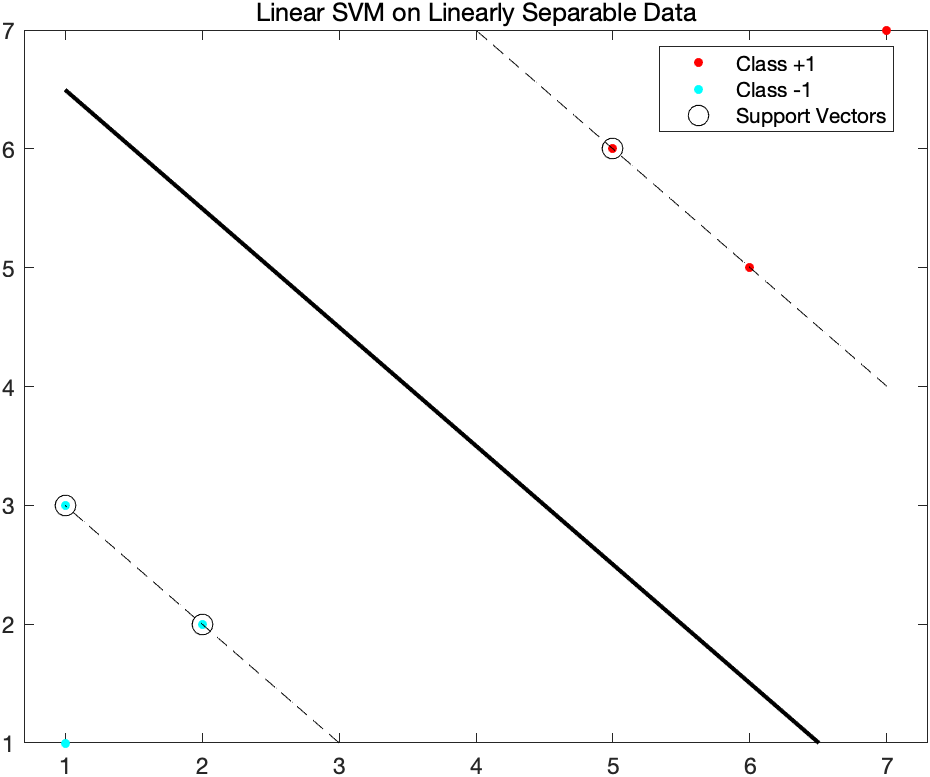
\includegraphics[width=0.72\textwidth]{figs/eg_hardSVM-plot.png}
%\caption{}
%\label{eg_softSVM-plot}
%\end{figure}
%

这个简单例子展示了 SVM 的一个重要特性：它只关注“最难分的样本”（即支持向量），从而形成一种稳健的决策边界。

这个例子展示了支持向量机“最大间隔 + 支持向量”的基本思想，以及如何从样本出发，推导出超平面的参数。尽管过程可以借助图形直观辅助，但更严谨的做法应采用对偶优化方法来计算准确的支持向量和参数。

\subsubsection{近似线性可分与软间隔 SVM}
% 引出软间隔和核方法的必要性
% 举例：现实中大多数问题是非线性可分的

假设你是某个社团的负责人，要将一批学生划分为“技术型”与“艺术型”两类。你根据他们的编程成绩和绘画作品评分来做判断。大多数学生的特征一目了然，可以清楚地分开，但有两个学生的表现就很尴尬：一个程序写得不错，但画画也很棒；另一个代码一塌糊涂，但绘画评分也偏低。

你现在面临的问题是：如果你坚持一刀切的分类标准（硬间隔），就不得不做出一些违心的决定。那有没有办法，在坚持“尽可能区分清楚”的前提下，允许少数点出错？

在上一节中，我们讨论了在理想情况下，训练数据在特征空间中是\textbf{线性可分}的，也就是说，存在一个超平面可以把正类与负类完全正确地分开，而且所有样本点都在各自类别的“间隔之外”。

然而，在现实世界中，数据往往不完美线性分离的。由于存在噪声（如图像识别中可能因光照或角度使图像模糊）、测量误差（如医学数据中存在测量误差或标签不一致）、类间重叠（如语言模型中句子语义模糊不清）等多种因素，使得某些样本难以被准确分离。
在这种情况下，硬性地要求“所有样本严格在其类别一侧---非此即彼”，往往会导致模型过拟合，泛化能力下降。

为此，支持向量机引入了一个关键的思想转变——\textbf{软间隔（Soft Margin）}：\textbf{允许部分样本点“越界”}，即位于其类别间隔内，甚至被误分类——只要总体分类边界尽可能宽，分类错误控制在合理范围内，模型就可以接受。

\paragraph{核心思想：放松刚性边界，换取更稳健的分类器}

为了量化“样本越界”的程度，SVM 为每个样本引入一个非负的\textbf{松弛变量（slack variable）} $\xi_i \geq 0$，表示样本~$x_i$偏离间隔边界的程度。于是，原先的硬间隔约束
$$
y_i \left( w^T x_i + b\right) \ge 1
$$
被放宽为
$$
y_i \left( w^T x_i + b\right) \ge 1-\xi_i
$$
同时，在优化目标中加入一个“惩罚项”，对所有“违反间隔”的样本进行惩罚。最终的优化目标函数变成了：
\begin{equation}\label{eq:soft_margin_primal}
\begin{aligned}
\min_{w,b,\xi} \quad & \frac{1}{2} \|w\|^2 + C \sum_{i=1}^n \xi_i \\
\text{s.t.} \quad & y_i(w^T x_i + b) \geq 1 - \xi_i, \quad \xi_i \geq 0, \quad i=1,\dots,n.
\end{aligned}
\end{equation}
其中的三个要素意义明确：
\begin{itemize}
\item 第一个目标项 $\frac{1}{2} \|w\|^2$ 仍然是最大化间隔；
\item 第二项 $C \sum_{i=1}^n \xi_i$ 对所有违反间隔约束样本的“误差惩罚项”；
\item 常数 $C > 0$ 是一个\textbf{正则化参数}，用来权衡“间隔最大化”与“分类误差最小化”之间的矛盾。
\end{itemize}

与硬间隔类似，软间隔 SVM 的求解也可借助对偶问题。不同的是，此时拉格朗日乘子的约束变为：
$$
0\le \alpha_i \le C 
$$
这个上界约束正体现了“软间隔”的精髓：既限制过度依赖某些误分类样本，又允许其在可控范围内对模型产生作用。

通过二次规划算法（如 SMO 算法）求解对偶问题， 得到乘子~$\alpha_i$，再反推出超平面参数~$w, b$。  满足 $0\le \alpha_i \le C $的样本称为{\bf 支持向量}，它们仍然是决定分类边界位置的关键点。

\eqref{eq:soft_margin_primal} 中的正则化参数{$C$ 是软间隔 SVM 中最关键的超参数之一，体现了模型对误分类的容忍程度：
\begin{itemize}
\item  若 $C$ 很大，模型对分类错误极度敏感，会试图避免任何越界或误分，这趋近于“硬间隔 SVM”的情形；
\item 若 $C$ 较小，模型更加关注整体间隔，容忍部分样本被误分类，从而获得更强的泛化能力。
\end{itemize}

通常， $C$  的选择方法包括：
\begin{itemize}
\item {\bf 经验设定：}先尝试默认值 $C=1$，再根据表现调整；这适合多数任务；

\item {\bf 交叉验证（cross-validation）：}在多个$C$ 值上训练模型，根据测试集准确率选择最佳者；

\item {\bf 网格搜索 + 验证集：} 在高维参数空间中配合验证集系统搜索。 
\end{itemize}

实际上，$C$  的调整如同转动一把“误差-间隔的调节旋钮”：太小，欠拟合；太大，过拟合；适中，正好平衡模型稳定性与鲁棒性。

从几何角度看，软间隔模型追求的是一种{\bf 容错鲁棒性}：不是力求“所有点都正确”，而是“整体效果最优”。

软间隔 SVM 实现了从“严格可分”到“容错分类”的平滑过渡，是处理现实数据不可或缺的工具。
即使某些点不在理想区域，SVM 也能通过“整体最优”的策略构造出更鲁棒的边界。

%硬间隔 SVM 无法容忍任何分类错误，会为了正确分类所有点而“牺牲”整体的间隔，导致边界扭曲。这将导致间隔变小、支持向量变多，最终带来的是模型的过拟合：它在训练集上“无懈可击”，但在新样本上却表现不佳。
%
%而软间隔 SVM 则采取了更灵活的策略：它允许 $(3, 2.5)$ 这个点\textbf{违反分类间隔约束}，甚至被误分（即它的松弛变量 $\xi_i > 1$），但整体决策边界仍然维持在一个尽可能稳健的位置上。如此一来，模型更关注“大多数样本的整体结构”，而非对“个别异常”的强制妥协，从而保持良好的泛化能力。

软间隔的引入不仅提高了模型的容错能力，也为后续核方法处理非线性问题奠定了数学基础。正因如此，它已成为工业界最主流的 SVM 实现方式之一。

\subsubsection*{例1：软间隔 SVM 分类示意 } 

为更直观理解软间隔 SVM 的动机与作用，我们来看一个简单的二维分类示例。
考虑如下二维数据集，其中包含 6 个样本：
\begin{center}
\begin{tabular}{cccc}
\toprule
$x_1$ & $x_2$ & 类别  &\\
\midrule
1 & 2 & A（+1）& \\
2 & 2 & A（+1）& \\
2 & 3 & A（+1）& \\
4 & 2 & B（-1）& \\
5 & 2 & B（-1）& \\
4.1 & 2.4 & A（+1）& $\quad\Rightarrow$ 噪声点（疑似异常） \\
\bottomrule
\end{tabular}
\end{center}

将这些样本点绘制在二维平面上，如图~\ref{eg_softSVM2} 所示。可以看出，大部分正类点主要分布在左边，大部分负类点主要分布在右边，第六个点 $(4.1, 2.4)$也是正类点，但位置比较靠近负类一侧，可能是标注错误、测量误差或特征扰动造成的异常值。

\begin{figure}[htbp]
\begin{subfigure}{0.49\linewidth}
\centering
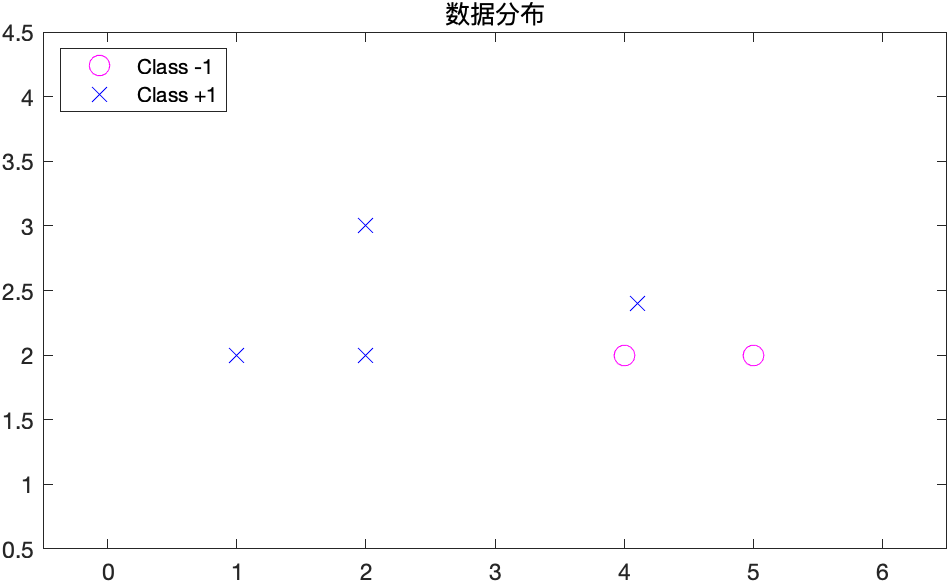
\includegraphics[width=1\textwidth]{figs/eg_softSVM1.png}
\caption{两类数据样本（软间隔） }
\label{eg_softSVM2}
\end{subfigure}
\begin{subfigure}{0.49\linewidth}
\centering
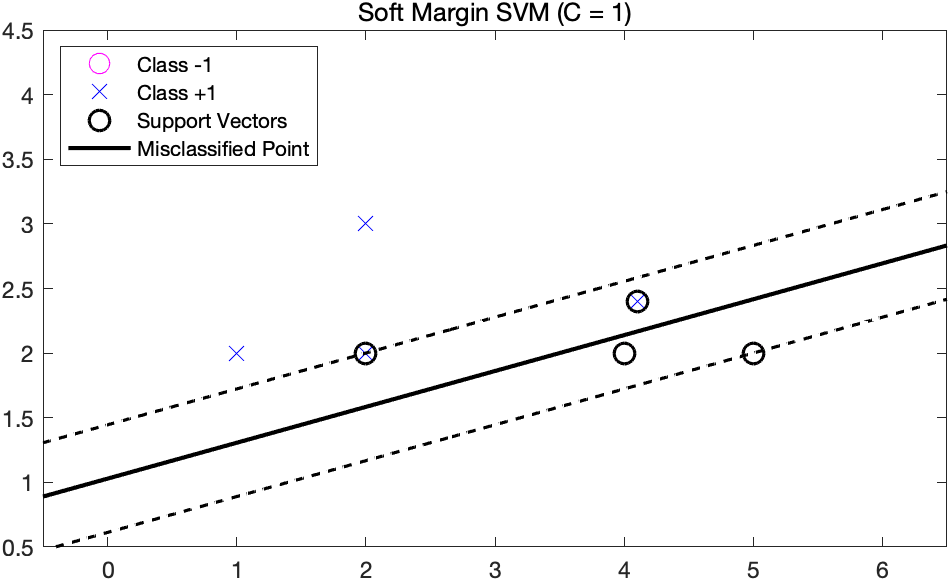
\includegraphics[width=1\linewidth]{figs/eg_softSVM1-C1.png}
\caption{正则参数~$C=1$}
\label{eg_softSVM1-正则参数1}
\end{subfigure}
\begin{subfigure}{0.49\linewidth}
\centering
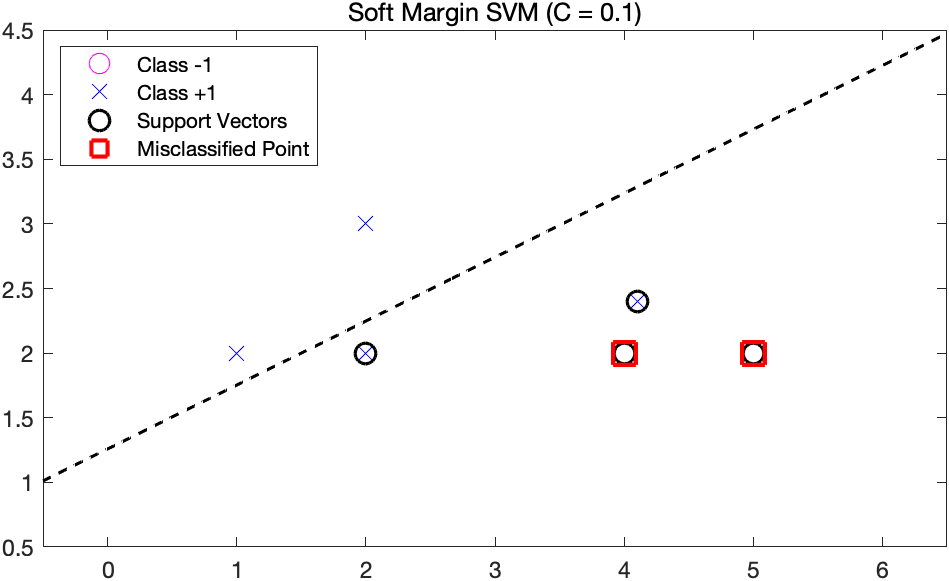
\includegraphics[width=1\textwidth]{figs/eg_softSVM1-C0.1.png}
\caption{正则参数~$C=0.1$}
\label{eg_softSVM1-正则参数0.1}
\end{subfigure}
\begin{subfigure}{0.49\linewidth}
\centering
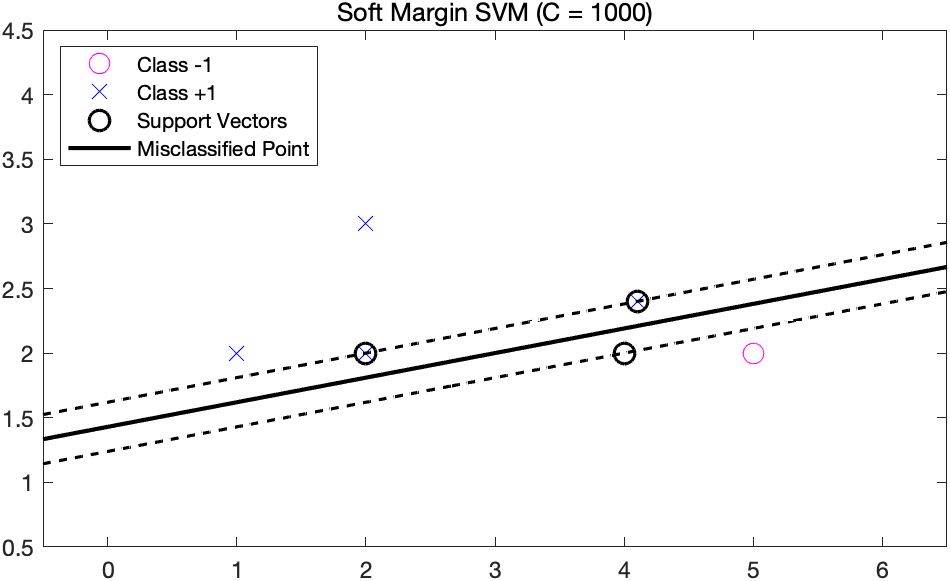
\includegraphics[width=1\textwidth]{figs/eg_softSVM1-C1000.png}
\caption{正则参数~$C=1000$}
\label{eg_softSVM1-正则参数1000}
\end{subfigure}
\caption{软间隔 SVM 分类示例一}
\label{软间隔 SVM 分类示例一}
\end{figure}
%
%\begin{figure}[htbp]
%\centering
%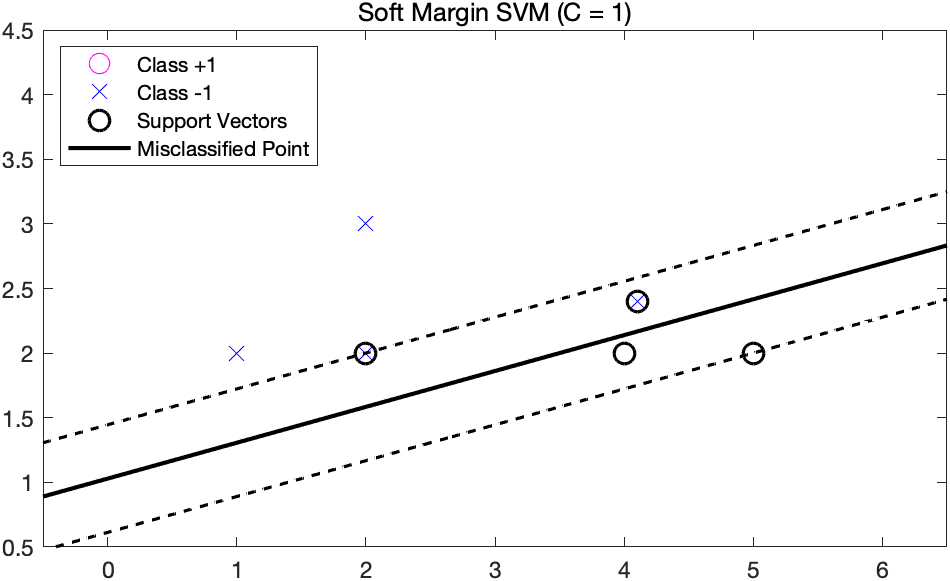
\includegraphics[width=0.72\textwidth]{figs/eg_softSVM4-C1.png}
%\caption{软间隔 SVM 分类示意图：$C=1$， 误分点 $(3, 2.5)$ 落在负类一侧，模型仍保持较大间隔。
%模型尝试兼顾间隔和分类精度，边界略微偏移。}
%\label{软间隔 SVM 分类示意图：$C=1$， 误分点 $(3, 2.5)$ 落在负类一侧，模型仍保持较大间隔。}
%\end{figure}

两类样本点在不同超参数~$C$值下的软间隔如图~\ref{软间隔 SVM 分类示例一}(b)-(c)所示，其中黑色实线代表分类决策边界 $w^T x + b = 0$， 黑色虚线代表间隔边界，用黑圈标出的样本点是支持向量。

如图~\ref{eg_softSVM1-正则参数1}，当正则参数~$C=1$时，模型在“误差惩罚”与“间隔保持”之间取得相对均衡，虽然仍容许部分点如 $(4.1, 2.4)$ 和$(4, 2)$ 落在间隔之内，但边界形状更加贴合数据分布。
    
而当正则参数~$C=0.1$时，如图~\ref{eg_softSVM1-正则参数0.1}，模型对误分容忍度较高，更关注整体的间隔最大化。结果中，虽然点 $(4.1, 2.4)$ 和 $(5, 2)$ 被误分为正类，但决策边界整体平稳、间隔较大。

当正则参数~$C=1000$时，如图~\ref{eg_softSVM1-正则参数1000}，模型几乎不容忍分类错误，尽力将所有点都分类正确，导致决策边界被迫贴近正类区域，间隔明显缩小，看上去“紧张兮兮”。

通过比较不同 $C$ 值下的结果可以看出，\textbf{正则化参数 $C$ 实质上控制了 SVM 的“严格程度”}：越大越严格，越小越宽容。选择合适的 $C$，才能平衡好误差容忍与模型鲁棒性的矛盾，使 SVM 在实际数据上获得更好的泛化表现。

在软间隔 SVM 中，支持向量的定义为满足 $0 < \alpha_i < C$ 的样本。支持向量的几何含义在软间隔中得以延续：\textbf{它们仍然是决定超平面位置的关键点}。根据样本违反间隔约束的程度，支持向量可能
\begin{itemize}
\item 正好落在间隔边界上（$\xi_i = 0$）; 
\item 处于间隔内部但未被误分类（$0 < \xi_i < 1$），即越界但仍分类正确;
\item 被误分类，即（$\xi_i > 1$）。
\end{itemize}

无论处于哪种状态，支持向量始终是模型学习的“关键证据”，它们直接影响决策边界的关键点。

\subsubsection*{例2：软间隔 SVM 分类示意 } 

为更直观理解软间隔 SVM 的动机与作用，我们来看一个简单的二维分类示例。
考虑如下二维数据集，其中包含 13 个样本：

\begin{center}
\begin{tabular}{cccc}
\toprule
$x_1$ & $x_2$ & 类别  & \\
\midrule
1 & 3 & A（+1） & \\
2 & 2.5 & A（+1）&  \\
1.5 &2 & A（+1）  &\\
2 & 3.5 & A（+1） & \\
3 & 3 &  A（+1）  &\\
4 &3.5 & A（+1）&\\
5 & 2 &  A（+1）& outlier \\
\midrule 
6 & 1 &  B（-1）&\\
7 & 1.5 &  B（-1）&\\
6.5 & 2 &  B（-1）&\\
7.5 & 2.5 &  B（-1）&\\
8 & 1.8 &  B（-1）&\\
3.5 & 3.5 &  B（-1）& outlier\\
\bottomrule
\end{tabular}
\end{center}

\begin{figure}[htbp]
\begin{subfigure}{0.49\linewidth}
	\centering
	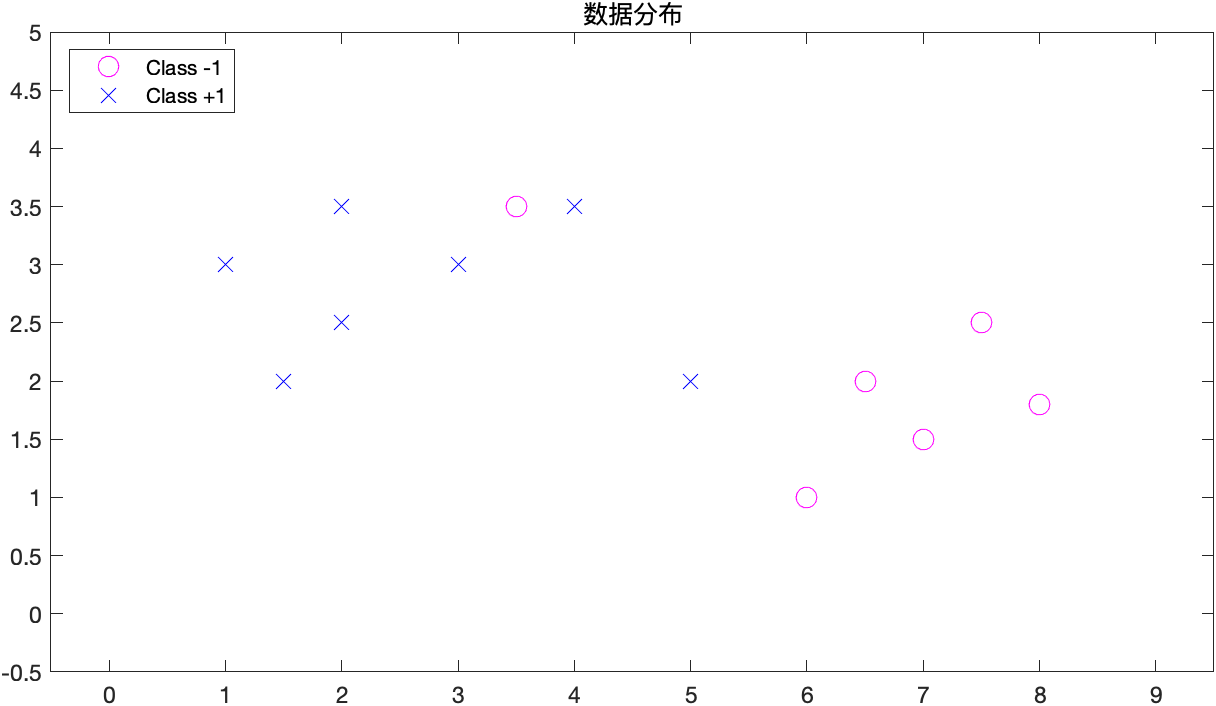
\includegraphics[width=1\textwidth]{figs/eg_softSVM2.png}
	\caption{两类数据样本}
	\label{eg2_softSVM2}
\end{subfigure}
\begin{subfigure}{0.49\linewidth}
	\centering
	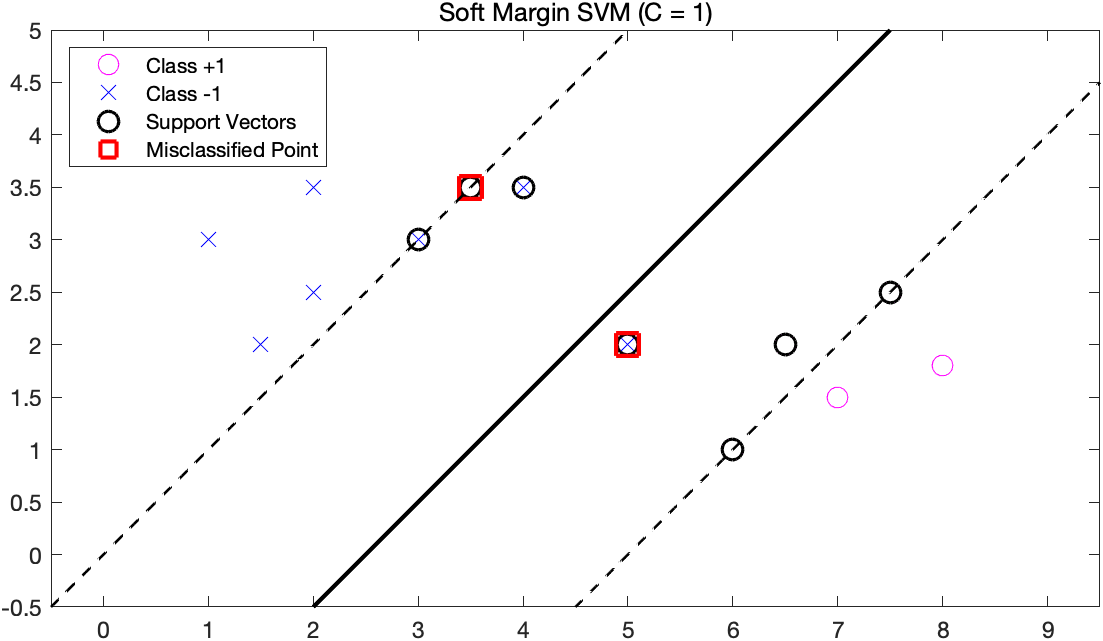
\includegraphics[width=1\linewidth]{figs/eg_softSVM2-C1.png}
	\caption{正则参数~$C=1$}
	\label{eg2_softSVM2-正则参数1}
\end{subfigure}
\begin{subfigure}{0.49\linewidth}
	\centering
	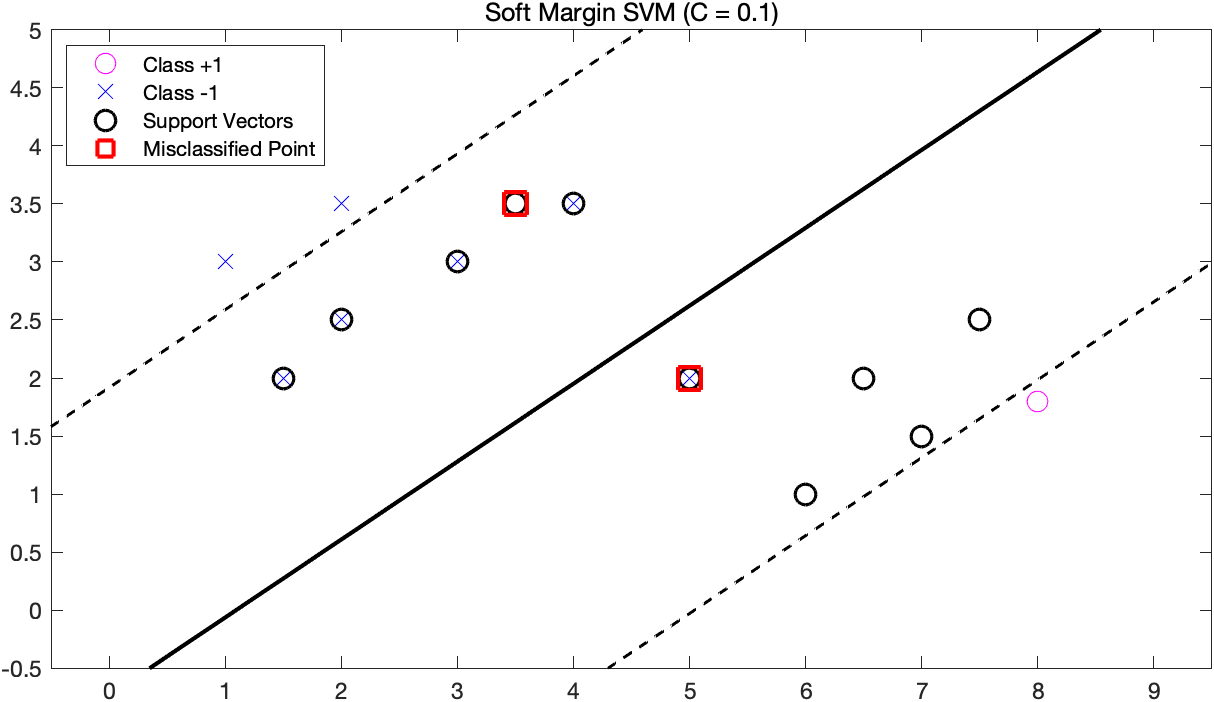
\includegraphics[width=1\textwidth]{figs/eg_softSVM2-C0.1.png}
	\caption{正则参数~$C=0.1$}
	\label{eg2_softSVM2-正则参数0.1}
\end{subfigure}
\begin{subfigure}{0.49\linewidth}
	\centering
	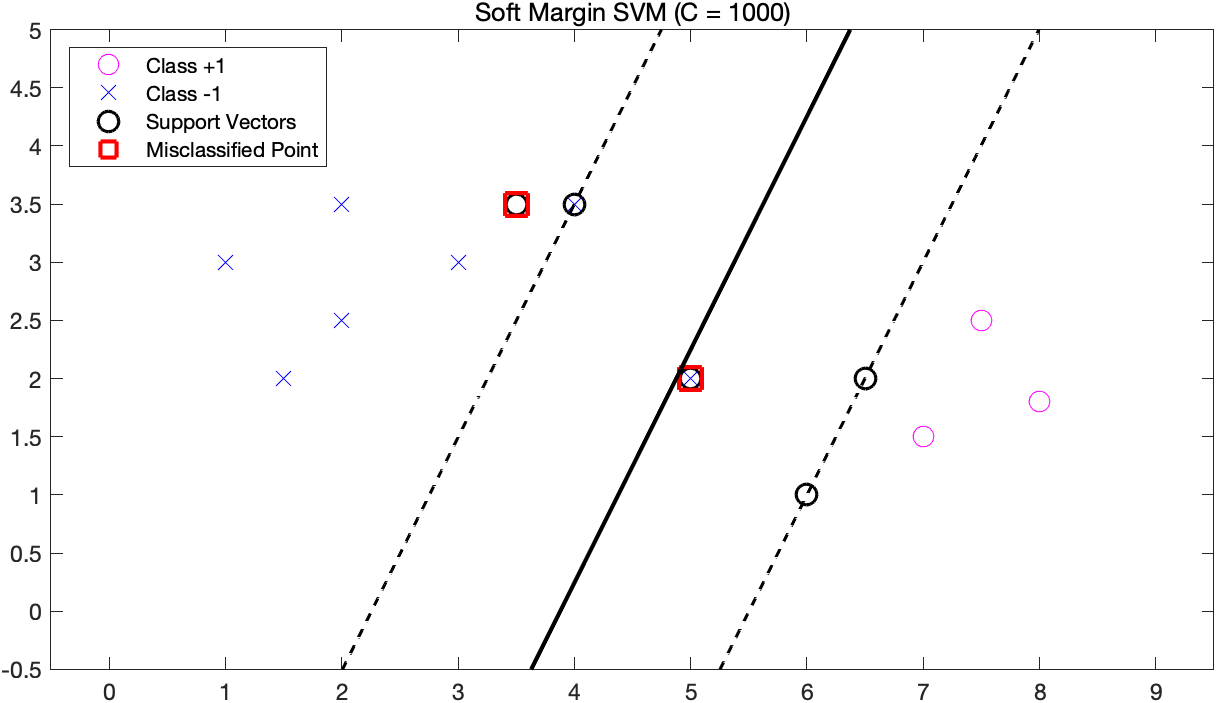
\includegraphics[width=1\textwidth]{figs/eg_softSVM2-C1000.png}
	\caption{正则参数~$C=1000$}
	\label{eg2_softSVM2-正则参数1000}
\end{subfigure}
\caption{软间隔 SVM 分类示例二}
\label{软间隔 SVM 分类示例二}
\end{figure}

将这些样本点绘制在二维平面上，如图~\ref{eg2_softSVM2} 所示。可以看出，大部分正类点主要分布在左上角，而大部分负类点主要分布在右下角，但有两个离群点~$(5,2)$ 和~$(3.5,3.5)$——它们是我们有意设置的误分类点。 

两类样本点在不同超参数~$C$值下的软间隔如图~\ref{软间隔 SVM 分类示例二}(b)-(c)所示，其中黑色实线代表分类决策边界 $w^T x + b = 0$， 黑色虚线代表间隔边界，用黑圈标出的样本点是{\bf 支持向量}。

我们比较三个不同的超参数~$C$值下的分类效果。当正则参数~$C=1$时， 如图~\ref{eg2_softSVM2-正则参数1}，模型在“误差惩罚”与“间隔保持”之间取得相对均衡，虽然仍容许部分点如~$(3.5,3.5),(2,3.5),(8, 1.8)$落在间隔之内，其中两个点（如 $(5, 2)$和~$(3.5,3.5)$ 被误分类。    

如图~\ref{eg2_softSVM2-正则参数0.1}，当正则参数~$C=0.1$时，模型对误分容忍度较高，更关注整体的间隔最大化。结果中，13个样本点中除了~$(1,3),(4,3.5),(5, 2)$ 之外，其余10个样本点都落在间隔之内，且$(3.5, 3.5)$ 和 $(5, 2)$ 被误分类，但决策边界整体平稳、间隔较大。

当正则参数~$C=1000$时，如图~\ref{eg2_softSVM2-正则参数1000}，决策边界的间隔明显缩。

通过比较不同 $C$ 值下的结果可以看出，\textbf{正则化参数 $C$ 实质上控制了 SVM 的“严格程度”}：越大越严格，越小越宽容。选择合适的 $C$，才能平衡好误差容忍与模型鲁棒性的矛盾，使 SVM 在实际数据上获得更好的泛化表现。

有趣的是，如图所示，即使将软间隔中的惩罚参数 $C$ 设置得非常大，我们也无法“逼近”一个完全的硬间隔模型。这说明，软间隔 SVM 并不是“硬间隔的近似解”，而是一种独立的优化目标：在容错和间隔之间寻找平衡。

软间隔 SVM 实现了从“严格可分”到“容忍错误”的平滑过渡，让 SVM 在面对现实世界数据时更加实用与鲁棒。

\subsubsection{非线性情形与核技巧——如何让不可分数据变得线性可分？}

非线性可分情形：核函数与高维映射的巧妙结合

在前一节，我们探讨了线性可分和近似线性可分情形下支持向量机的最大间隔原理。
但在实际应用中，很多数据在原始空间中并不是线性可分的，而是呈现出明显的非线性特征——比如同心圆状、螺旋状、交错分布等。这种情况下，简单的线性超平面就无法胜任分类任务了。

考虑一个经典的“同心圆”数据集。如图~\ref{eg_nonlinearSVM}所示， 类别 A(蓝色点) 分布在图像中心，类别 B (红色点)环绕在外围形成一个环。显然，它们在原始的二维平面中无法被一条直线分开。
\begin{figure}[htbp]
\centering
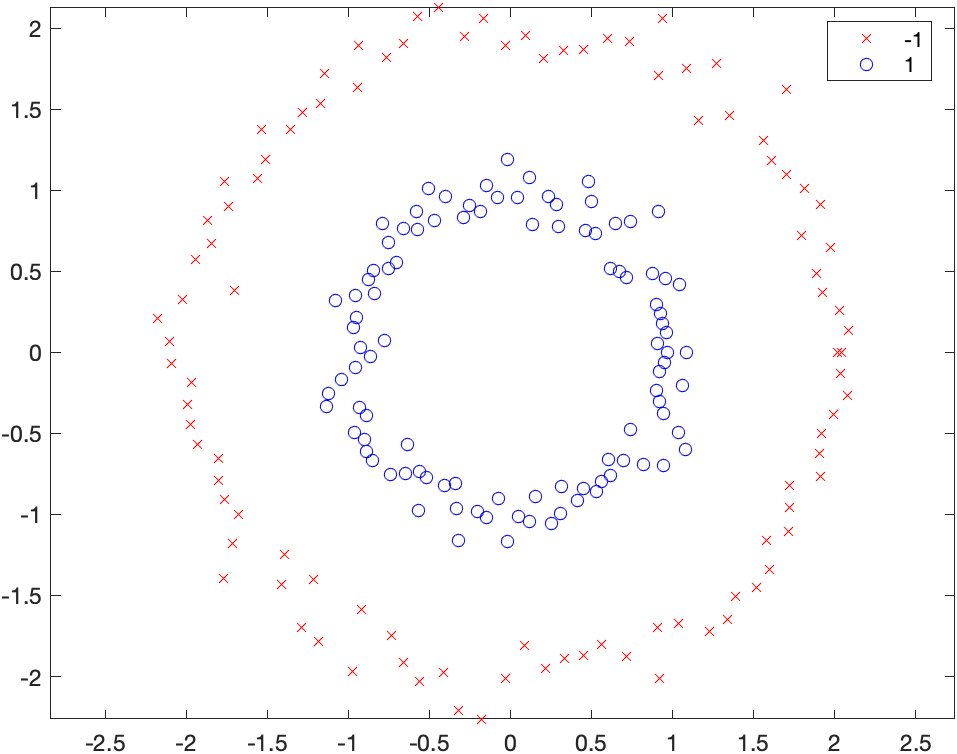
\includegraphics[width=0.72\textwidth]{figs/eg_nonlinearSVM.png}
\caption{}
\label{eg2_softSVM-plot}
\end{figure}

面对“线性不可分”的数据，支持向量机提供了一个优雅的解决方案---\textbf{升维再线性分类}。

%> \emph{将原始输入数据通过非线性映射 $\phi(x)$映射到高维空间，在高维空间中变为线性可分，然后在这个高维空间中应用线性SVM。}
%
%这就好比我们面对一个用直线分不开的圆形分布点（如内圈为一类，外圈为另一类），我们无法在二维空间中用线分开它们，但在三维空间中却可以用一个平面将它们一刀两断。

\paragraph{升维背后的数学思想}
假设我们有一个非线性映射 $\phi(x)$，它能把数据从原始空间 $\mathbb{R}^d$ 映射到高维空间 $\mathcal{H}$
\[
\phi: \mathbb{R}^d \rightarrow \mathcal{H}, \quad x \mapsto \phi(x)
\]
使得在高维空间~$\mathcal{H}$中，原本无法线性分开的数据可能变得线性可分，从而可以应用线性 SVM。

但这里面有一个实际难题~$\mathcal{H}$的\textbf{维度太高甚至无限维}，从而使得计算代价太高。

SVM的聪明之处在于：我们并不需要显式地计算~$\phi$，只需要引入一个“核函数”
\begin{equation}\label{kernel_func}
K({ x}, {x}^\prime) = \langle \phi({x}), \phi({x}^\prime) \rangle=\phi({ x})^T\phi({ x}^\prime) 
\end{equation}
核函数 $K(x, x^\prime)$ 本质上是一个内积运算，直接计算原始数据映射后的内积，把“升维”和“分类”打包进了一个快捷键里：

> \textit{只要选好核函数，系统就自动帮你完成了升维和分类的所有计算。}


最后，我们将视线聚焦到SVM的对偶问题本身上来。回顾线性可分情形下支持向量机的对偶优化问题具有如下形式：
\begin{equation*}
\begin{array}{c}
{\rm max}_{\alpha} \sum_{i=1}^6 \alpha_i -\frac{1}{2} \sum_{i=1}^6 \sum_{j=1}^6 \alpha_i \alpha_j y_i y_j {\bf x}_i^T {\bf x}_j \\
{\rm s.t.} \;  \sum_{i=1}^6 \alpha_i y_i =0 \\
\alpha_i \ge 0, \forall i=1, \dots, 6 
   \end{array}
\end{equation*}

在上述对偶优化问题中，最核心的运算是数据样本之间的内积，即形如：
\[
\phi(x_i)^T \phi(x_j)
\]
这样的表达式。这实际上意味着，在分类决策过程中，我们只关心数据点之间的相似程度，而不是数据本身具体在高维空间中的位置。

如前所述，我们可以用核函数替换上述的内积计算 $\phi(x_i)^T \phi(x_j)$。
借助核函数，我们再也不需要显式地知道数据被如何映射到高维空间，只需要通过核函数的简单计算，即可在原始空间内高效地完成高维空间的内积运算。这种技巧大幅简化了计算复杂度，极大扩展了SVM在实际应用中的可行性和灵活性。

如此一来，分类决策函数就优雅地变成：
\[
f(x) = {\rm sign}\left(\sum_{i=1}^n \alpha_i y_i K(x_i, x) + b \right)
\]
在这个最终的表达式里，\(\alpha_i\) 表示支持向量对应的权重，\(y_i\) 是对应支持向量的类别标签，而核函数 \(K(x_i,x)\) 则直接捕获了测试数据点 \(x\) 与每个支持向量 \(x_i\) 在隐含高维空间中的相似度。通过这样的方式，我们轻松实现了复杂非线性边界的分类任务。

%非线性可分问题的核SVM求解步骤如下：
%\begin{enumerate}
%\item {\bf  非线性映射：}设原始特征为 $x \in \mathbb{R}^d$，通过一个非线性函数 $\phi(x)$ 映射到高维空间 $\mathcal{H}$。
%
%\item {\bf 核函数替代内积：}为了避免直接在高维空间计算（维度太高甚至无限），我们使用核函数 $K(x_i, x_j) = \langle \phi(x_i), \phi(x_j) \rangle$ 计算“映射后的内积”。
%
%\item\end{enumerate}

\subsubsection{常见核函数：不同的升维效果}


使用多项式核函数：
\[
K(x, x') = (\langle x, x' \rangle + 1)^2
\]
或高斯径向基核函数（RBF）：
\[
K(x, x') = \exp\left(-\frac{\|x - x'\|^2}{2\sigma^2}\right)
\]


\begin{table}[htbp]
\centering
\caption{常用核函数及其特性}
\begin{tabular}{|c|c|p{7cm}|}
\hline
\textbf{核函数} & \textbf{表达式} & \textbf{特点} \\
\hline
线性核 & $\langle x, x' \rangle$ & 不升维，适合原始空间可线性分的数据 \\
\hline
多项式核 & $(\langle x, x' \rangle + c)^d$ & 模拟多项式映射，可处理曲线边界；$d$ 控制非线性程度 \\
\hline
高斯核（RBF） & $\exp\left(-\frac{\|x - x'\|^2}{2\sigma^2}\right)$ & 将数据映射到无限维空间，适合高度非线性分布，分类边界柔软灵活 \\
\hline
Sigmoid 核 & $\tanh(\alpha \langle x, x' \rangle + c)$ & 类似神经网络中的激活函数，非凸性限制了其使用场景 \\
\hline
\end{tabular}
\label{tab:kernelfunctions}
\end{table}

\paragraph*{是否需要逐步升维？}
% 正好作为对“升维直觉”的澄清，以及对 kernel trick 的方法论解释

在实际应用中，SVM 并不会先判断数据是否在线性空间中可分，再逐层尝试升维。而是采用一种“\textbf{一步到位}”的策略：通过选择一个合适的核函数 \(K(\mathbf{x}, \mathbf{x}')\)，\textbf{直接将数据隐式映射到一个高维空间}中，期望在这个空间中数据是线性可分的。

由于核函数只计算样本对之间的内积，无需显式构造映射后的特征表示，因此也无法显式判断“是否成功线性可分”。通常，我们通过优化问题的可解性、模型在训练与验证集上的性能，\textbf{隐式判断}所选核函数是否合适。

因此，SVM 的实际流程并不是“先判断线性可分 → 不可分则升维”，而是“\textbf{直接选择一个可能让数据线性可分的核函数进行训练}”，再通过交叉验证等方法确定其有效性。

\paragraph{示例：双环分布（环形数据）}
考虑以下二维数据：

内圈为正类 $(+1)$，外圈为负类 $(-1)$；

在二维平面中显然无法用一条直线分开，但如果使用合适的核函数（如径向基核 RBF），就可以在高维空间找到一个分界超平面。



\paragraph*{一个非线性示例：核方法如何“化曲为直”}

\begin{figure}[htbp]
\centering
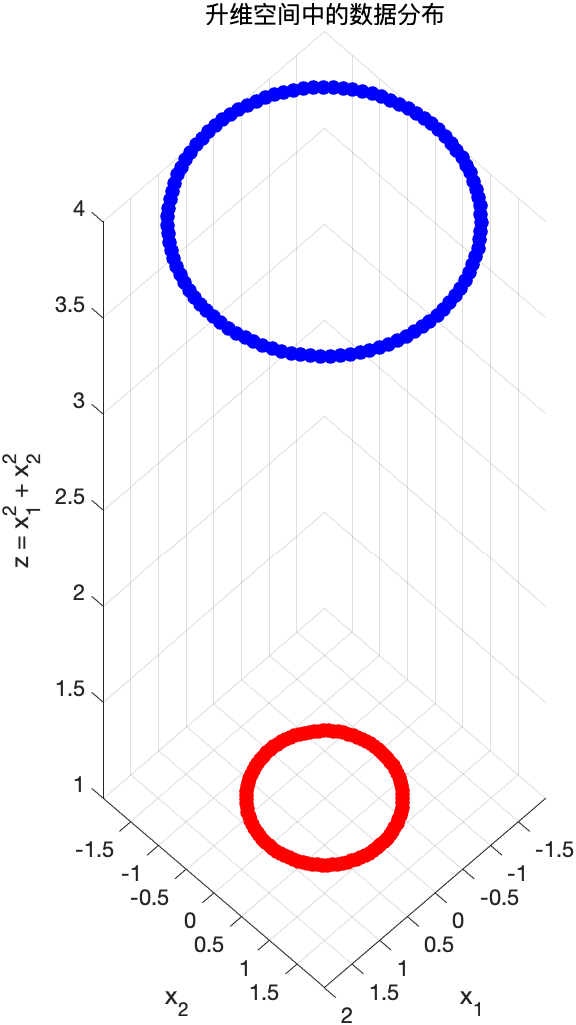
\includegraphics[width=0.4\textwidth]{figs/eg_kernel.png}
\caption{}
\label{eg_nonlinearSVM}
\end{figure}

\begin{figure}[htbp]
\centering
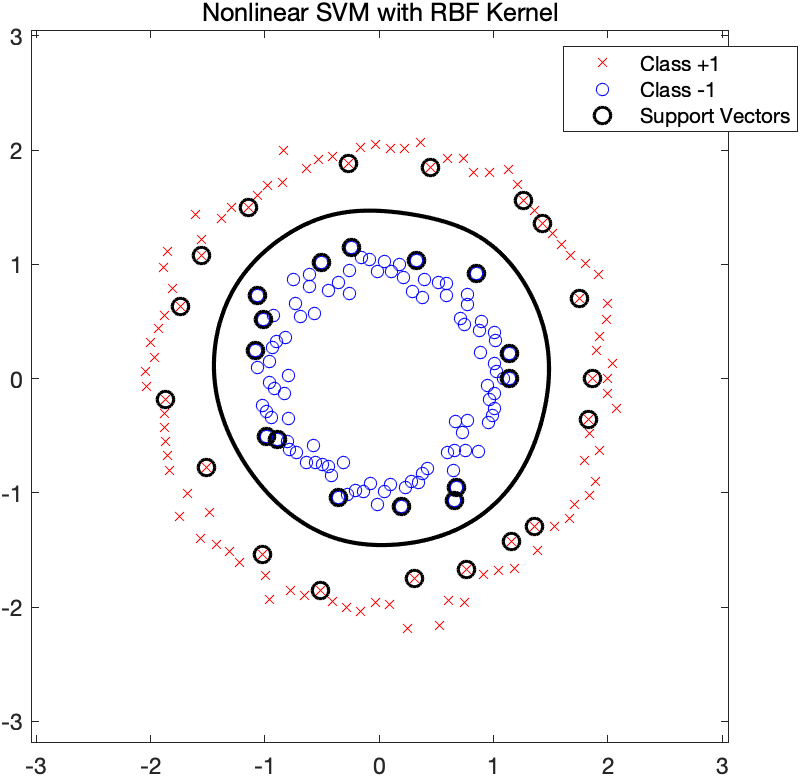
\includegraphics[width=0.72\textwidth]{figs/eg_nonlinearSVM-plot.png}
\caption{}
\label{eg_nonlinearSVM-plot}
\end{figure}

\begin{figure}[htbp]
\centering
\begin{subfigure}{0.49\linewidth}
\centering
\begin{tikzpicture}
\begin{axis}[
    axis lines=none,
    width=7cm, height=7cm,
    xtick=\empty, ytick=\empty,
    enlargelimits,
    clip=true
]
\addplot[only marks, mark=*, mark size=2pt, blue] table {
0.5 0
-0.5 0
0 0.5
0 -0.5
};
\addplot[only marks, mark=*, mark size=2pt, red] table {
1.5 0
-1.5 0
0 1.5
0 -1.5
1 1
-1 -1
};
\draw[dashed] (axis cs:0,0) circle [radius=1.2];
\end{axis}
\end{tikzpicture}
\caption{原始空间线性不可分的数据集}
\end{subfigure}
\begin{subfigure}{0.49\linewidth}
\centering
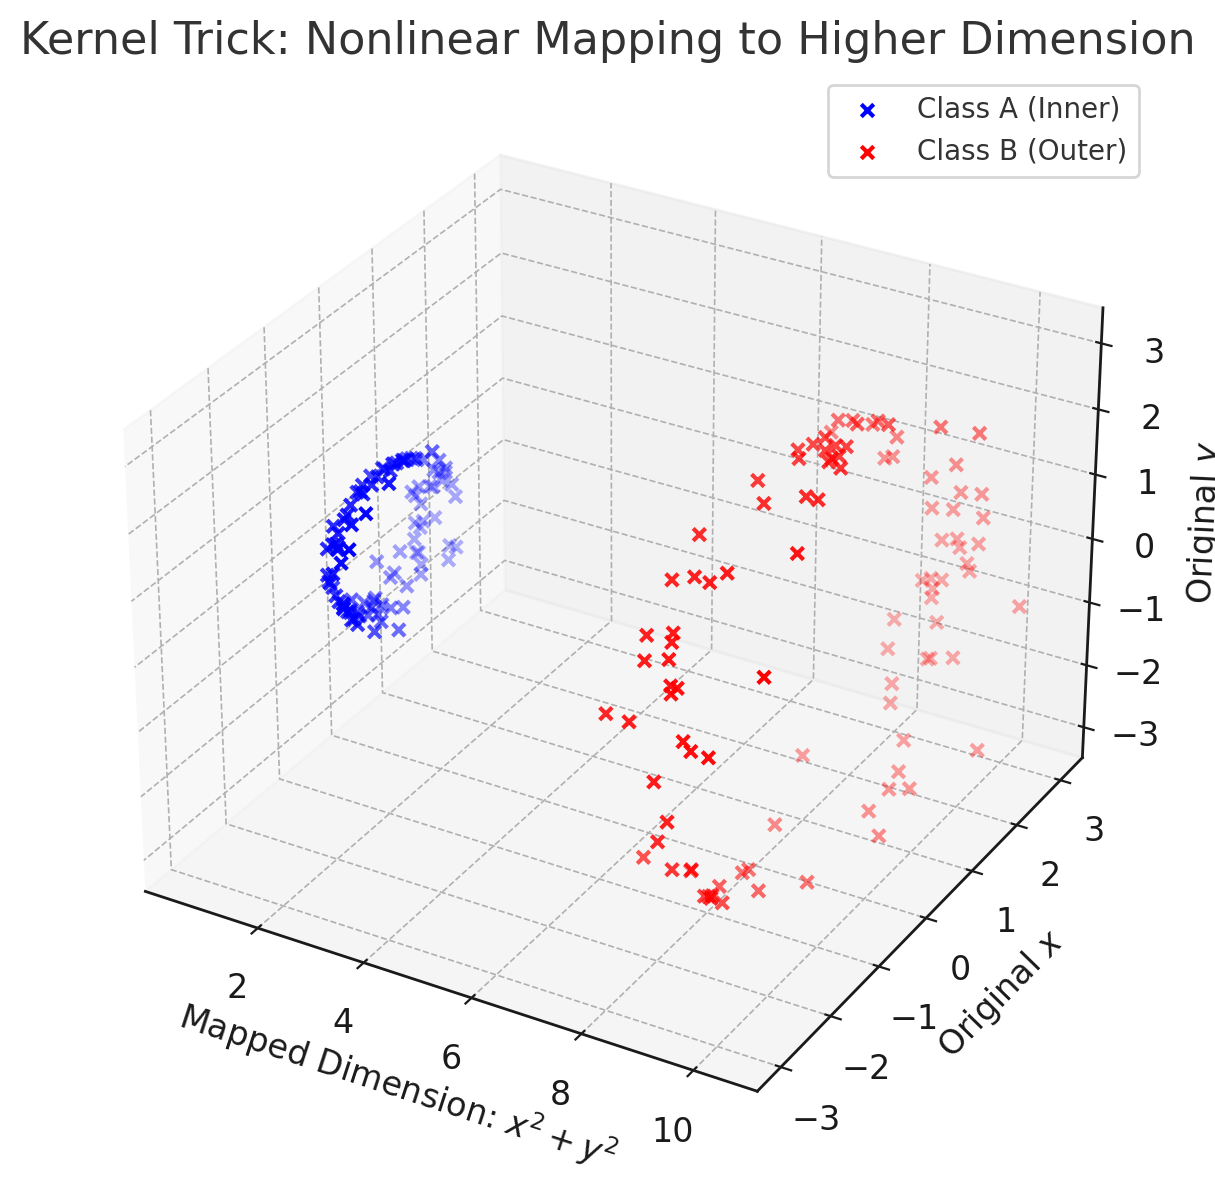
\includegraphics[width=0.9\textwidth]{figs/svm_kernel_curve.png}
\caption{在高维空间线性可分}
\label{在高维空间线性可分}
\end{subfigure}
\caption{非线性边界通过核方法在高维空间中实现线性分离}
\label{非线性边界通过核方法在高维空间中实现线性分离}
\end{figure}

\subparagraph*{核方法：升维处理}

我们可以使用核方法进行非线性映射：
\[
\phi(x_1, x_2) = x_1^2 + x_2^2
\]
即将数据从二维映射到一维的“半径平方”空间（实际上是内积空间中高维超平面），这样在新空间中就变成了线性可分，见图~\ref{在高维空间线性可分}
\subparagraph*{分类器在核空间中的效果}

经过核函数处理后，SVM 能在高维特征空间中找到一个超平面，从而在原空间中形成一个“非线性边界”（比如圆形、环形）来完成分类。


\subsection{升维示意图}

考虑将原始数据 \((x, y)\) 映射到三维空间，其中第三个维度是：
\[
z = x^2 + y^2
\]

这样，原本在二维空间中重叠的两个圆，就变成了在三维空间中处于不同高度的“平面”，从而可以通过一个平面（超平面）将其线性分割。


\subsection{核函数的数学形式}

这种升维对应于一种常见的核函数：\textbf{多项式核函数}：

\[
K(\mathbf{x}, \mathbf{x}') = (\mathbf{x} \cdot \mathbf{x}')^2
\]

这种核函数隐式地将原始输入空间中的数据点映射到包含二次项的高维特征空间，例如：

\[
(x_1, x_2) \mapsto (x_1^2, \sqrt{2}x_1 x_2, x_2^2)
\]

从而使原本线性不可分的数据，在新的空间中变得线性可分。


\paragraph{例子：同心圆数据的升维}
如下图所示：

\begin{itemize}
    \item 原始二维空间中，同心圆内外两类点线性不可分；
    \item 若将 $(x, y)$ 映射为 $(x^2 + y^2)$，则可以看成在三维空间中形成两个不同“高度”的平面；
    \item 在高维中，它们可被一个平面（超平面）分离；
\end{itemize}

这背后隐含的是一个形如 $\phi(x) = x_1^2 + x_2^2$ 的映射，或其对应的多项式核函数：
\[
K(x, x') = (\langle x, x' \rangle + 1)^2
\]

\subsubsection{从对偶问题到决策函数：核技巧的最终表达}

核函数被引入对偶问题后，SVM 的优化形式变为：

\begin{equation}
\max_\alpha \sum_{i=1}^n \alpha_i - \frac{1}{2} \sum_{i,j=1}^n \alpha_i \alpha_j y_i y_j K(x_i, x_j)
\end{equation}

对应的分类决策函数变为：

\begin{equation}
\boxed{
    f(x) = \mathrm{sign}\left(\sum_{i=1}^n \alpha_i y_i K(x_i, x) + b\right)
}
\end{equation}

\subsubsection{总结：核技巧为何如此强大？}

\begin{itemize}
    \item 它让你\textbf{不显式升维}就能获得升维的分类能力；
    \item 它将\textbf{复杂边界问题转化为超平面分类问题}；
    \item 它赋予 SVM 非凡的灵活性，适应各种复杂数据结构；
    \item 它将“内积”的概念推广为“相似度”，与后来的深度学习遥相呼应。
\end{itemize}

\begin{quote}
\itshape
“在低维中画不了线？那就升到高维划平面！”
\end{quote}


\subsection{不同核函数的升维效果比较}
你可以把原始数据映射到高维空间，在那个空间里再找超平面。而核函数的作用，就是{\bf 不显式映射也能计算高维空间内积}，节省了大量计算。

常见核函数包括：

- 线性核（Linear Kernel）：不升维，适合线性问题
- 多项式核（Polynomial Kernel）：能处理复杂曲线
- 高斯径向基核（RBF）：相当于“无限维”映射，强大到飞起；映射到无限维空间，适合高度非线性数据
-Sigmoid 核：与神经网络激活函数相似

核方法的引入，不仅扩展了 SVM 的应用范围，也对后来的深度学习中“特征空间映射”思想产生了深远影响。
\begin{table}[htbp]
\centering
\caption{不同核函数的升维效果与适用情境}
\begin{tabular}{|c|c|p{7cm}|}
\hline
\textbf{核函数类型} & \textbf{数学表达} & \textbf{特点与适用情况} \\
\hline
线性核 & \( K(\mathbf{x}, \mathbf{x}') = \mathbf{x} \cdot \mathbf{x}' \) & 不进行升维，适用于原始空间中线性可分的数据 \\
\hline
多项式核 & \( K(\mathbf{x}, \mathbf{x}') = (\mathbf{x} \cdot \mathbf{x}' + c)^d \) & 明确升维到多项式特征空间，适用于存在明显非线性边界的情形 \\
\hline
高斯核（RBF） & \( K(\mathbf{x}, \mathbf{x}') = \exp\left(-\frac{\|\mathbf{x} - \mathbf{x}'\|^2}{2\sigma^2}\right) \) & 相当于将数据映射到无限维空间，适用于复杂分布的数据，分类边界灵活 \\
\hline
\end{tabular}
\label{tab:kernel_comparison}
\end{table}


通过核函数，SVM 不需要显式地进行高维计算，而是利用核技巧在原始空间中计算内积，从而实现\textbf{隐式升维}。这种方式不仅高效，而且功能强大，广泛应用于文本分类、图像识别、生物信息等领域。

这个例子展示了核方法的强大之处：
\begin{itemize}
    \item 原空间非线性不可分 $\Rightarrow$ 映射到核空间后线性可分；
    \item 不需显式构造特征，只需设计好核函数；
    \item 支持向量机借助核技巧，能处理各种复杂的分类边界问题。
\end{itemize}

这就是所谓的：
\begin{quote}
\itshape
“在原空间划不了线，那就升维之后划平面。”
\end{quote}


 
 核函数的登场：无需显式升维的巧妙方法

显式地将数据映射到高维空间可能会带来巨大的计算成本。核函数就是为了解决这个问题而生的。它就像一个“魔术师”，能够直接计算高维空间中数据点之间的内积，而无需显式地执行升维操作。

 核函数的数学本质：内积与相似性

核函数 $k({\bf x}_i, {\bf x}_j)$ 的数学本质是计算两个数据点 ${\bf x}_i$ 和 ${\bf x}_j$ 在高维空间中的内积。内积是一个衡量向量相似性的指标。

-内积的几何意义： 两个向量的内积等于它们的长度之积乘以它们之间夹角的余弦值。
-内积的代数意义： 两个向量的内积等于它们对应分量乘积之和。

核函数的神奇之处在于，它能够直接计算高维空间中的内积，而无需知道映射函数 $\phi({\bf x})$ 的具体形式。这就像一个黑盒子，我们只需要输入两个数据点，它就能输出它们在高维空间中的相似度。

 常用的核函数及其数学特性

-多项式核函数： $k({\bf x}_i, {\bf x}_j) = ({\bf x}_i^T {\bf x}_j + c)^d$
    -- 它能够模拟多项式映射，将数据映射到多项式空间。
    --参数 $c$ 和 $d$ 控制着多项式的次数和偏移量。
-高斯核函数（RBF）： $k({\bf x}_i, {\bf x}_j) = \exp(-\frac{\|{\bf x}_i - {\bf x}_j\|^2}{2\sigma^2})$
   -- 它能够模拟无限维映射，将数据映射到一个无限维的希尔伯特空间。
    -- 参数 $\sigma$ 控制着高斯函数的宽度，影响着模型的复杂程度。
-Sigmoid 核函数： $k({\bf x}_i, {\bf x}_j) = \tanh(\alpha {\bf x}_i^T {\bf x}_j + c)$
    -- 它类似于神经网络中的激活函数，能够模拟神经网络的非线性映射。
    --参数 $\alpha$ 和 $c$ 控制着 sigmoid 函数的形状和偏移量。

 核函数的选择：一门艺术

选择合适的核函数是一个需要经验和技巧的过程。不同的核函数适用于不同的数据分布和问题类型。这就像选择一把合适的钥匙来打开一扇门，需要仔细考虑门的形状和锁的类型。

 核技巧在 SVM 中的应用

将核函数引入支持向量机的对偶问题 \eqref{eq:svm_opt}，我们可以得到：

\begin{equation}\label{eq:svm_kernel_opt}
\begin{array}{c}
{\rm max}_{\alpha} \sum_{i=1}^n \alpha_i -\frac{1}{2} \sum_{i,j=1}^n \alpha_i \alpha_j y_i y_j k({\bf x}_i, {\bf x}_j) \\
{\rm s.t.} \; \alpha_i \ge 0, \forall i=1, \dots, n \\
\; \sum_{i=1}^n \alpha_i y_i =0
\; \end{array}{c}
\end{equation}

决策函数变为：

\begin{equation}\label{eq:svm_kernel_decision}
f({\bf x}) = {\rm sign}\left(\sum_{i=1}^n \alpha_i y_i k({\bf x}_i, {\bf x}) + b\right)
\end{equation}

通过核技巧，我们可以将支持向量机从线性模型扩展到非线性模型，从而处理更加复杂的数据分布。

 总结

支持向量机的非线性可分与核函数是一个充满智慧和创造力的领域。通过升维和核函数，我们能够处理复杂的非线性问题，让机器学习模型更加强大。

\paragraph*{优点与局限：曾经的王者，如今的利器}
{四、泛化能力与优势：它为何经典？}
SVM 不仅在训练集上表现良好，更重要的是它具备优秀的泛化能力，也就是说，它在没见过的数据上也能表现稳定。

为什么？关键在于它最大化了间隔。这种设计天然抑制过拟合，就像考试时“坐在教室中间最安全”的那个同学，能避免很多边界情况。

SVM 的优点总结如下：
-几何直观：最大间隔让人一眼明了
- 支持非线性分类（通过核函数）
- 理论基础扎实，优化问题凸、解唯一
可解释性强：支持向量一目了然
-对小样本、高纬度场景下表现优秀：在样本数量少但特征维度高时表现佳
- 鲁棒性好：对噪声不敏感（尤其在硬间隔设定下）


\paragraph*{五、局限与转型：老将不退，转战新阵地}
当然，SVM 也不是万能的。它的主要局限包括：

对参数敏感（如正则项 C 和核函数选择）

对大数据不够友好：训练时间随样本数呈平方增长

主要用于“判别问题”，难以用于生成式建模

在多类分类问题中需要“一对一”或“一对多”扩展，结构复杂

因此，在图像、语音等大数据场景中，SVM 逐渐被深度学习取代。但在结构清晰、数据有限、特征表达明确的任务中，它依然是“轻巧、可靠的老将”。

局限：
- 在大规模数据上计算开销大
- 对参数（如核函数、正则系数）较敏感，需调参
- 在深度学习兴起后，逐渐在图像、语音等领域被取代

\paragraph*{SVM 的思维遗产}

虽然在实际应用中 SVM 逐渐退居二线，但它留下了重要的“思维遗产”：
- 最大间隔的思想，影响了后来的分类方法
- 核技巧启发了后来的非线性特征映射思路
- 可解释性与理论优雅，依然是很多学术模型的参考标准

 在机器学习的历史长河中，SVM 是一位“功成身退”的老将，它的经典之处在于：用几何之美，划分复杂世界。

支持向量机告诉我们，机器学习不仅是计算，更是一种关于边界、结构与余地的哲学。



%\end{appendixsection}


\subsection{ 无监督学习 (Unsupervised Learning)：通过未标注数据发现模式}

与监督学习相反的是，非监督学习（Unsupervised Learning）所处的学习环境，都是非标签的数据。韩家炜教授接着说\cite{han2011data}，

“非监督学习，本质上就是‘聚类（Cluster）’的近义词。”

无监督学习是一种无需标签数据的机器学习范式，其核心目标是从未标注的输入数据中挖掘潜在的结构或模式。这种学习方式在数据探索、特征提取、模式发现等领域有着广泛的应用。

在无监督学习中，训练数据仅包含输入 $X$，而没有对应的标签 $Y$。模型通过分析输入数据的分布特征，发现潜在的模式或分布规律。由于缺乏明确的标注，模型通常基于数据的内在关系（如相似性或分布密度）来进行训练和推断，进而实现任务目标。

话说聚类的思想起源非常早，在中国，可追溯到《周易\textperiodcentered 系辞上》中的“方以类聚，物以群分，吉凶生矣”。

但真正意义上的聚类算法，却是20世纪50年代前后才被提出的。

为何会如此滞后呢？原因在于，聚类算法的成功与否，高度依赖于数据。数据量小了，聚类意义不大。数据量大了，人脑就不灵光了，只能交由计算机解决，而计算机1946年才开始出现。

如果说分类是指，根据数据的特征或属性，划分到已有的类别当中。
那么，聚类一开始并不知道数据会分为几类，而是通过聚类分析将数据聚成几个群。

简单来说，给定数据，聚类从数据中学习，能学到什么，就看数据本身具备什么特性了（given data, learn about that data）。
%----
%无监督学习的分类依据
无监督学习的理论基础建立在一个核心假设上：{\bf 相似样本在数据空间中的距离通常较近}。这一假设引导算法通过度量样本之间的相似性或差异性，揭示数据的结构和分布规律。
这一假设可以分为两大原则：
\begin{itemize}
\item {\bf 类内相似性}  属于同一类别的样本往往表现出特征上的一致性，其分布在数据空间中相对集中。例如，图像数据中的相似物体、文本数据中的同义表达等。
\item {\bf 类间差异性}  不同类别的样本之间具有显著的差异性，表现为在特征空间中的分布距离较远。这使得数据可以自然地划分为多个互不重叠的组。
\end{itemize}

对此，北京航空航天大学的于剑教授，对聚类有12字的精彩总结[2]：
“归哪类，像哪类。像哪类，归哪类。”
展开来说，给定N个对象，将其分成K个子集，使得每个子集内的对象相似，不同子集之间的对象不相似。

但这里的“类”也好，“群”也罢，事先我们是并不知情的。一旦归纳出一系列“类”或“群”的特征，如果再来一个新数据，我们就根据它距离哪个“类”或“群”较近，就预测它属于哪个“类”或“群”，从而完成新数据的“分类”或“分群”功能。

典型的无监督学习任务包括聚类分析、降维、关联分析、异常检测和生成模型等。

聚类分析旨在将数据集划分为若干组（即簇），使得每组内的样本具有高度相似性，而不同组之间的样本差异显著。常见算法包括K均值聚类、层次聚类、密度聚类（如DBSCAN）等，应用场景则涵盖用户分群、文本聚类、图像分割等领域。例如，在市场细分中，将顾客分为多个群体，根据其购买行为进行个性化推荐。

降维通过减少特征的维度来简化数据表示，同时尽量保留关键信息。常见方法包括主成分分析（PCA）、t-SNE、线性判别分析（LDA）等。应用场景涵盖 数据可视化、特征压缩、降噪等。例如，将高维基因表达数据映射到二维空间以便于观察聚类结构。

关联分析用于发现数据中变量之间的潜在关联关系。经典案例包括 超市购物者常同时购买啤酒和尿布的“啤酒与尿布”关联规则。更多应用场景包括 市场篮分析、推荐系统、商业决策。常用算法包括 Apriori 和 FP-Growth。

异常检测通过识别数据中偏离正常模式的样本来发现异常点。其核心思想是，异常样本往往位于分布的稀疏区域或具有不寻常的特征值。异常检测通常应用于 信用卡欺诈检测、网络入侵检测、设备故障诊断等领域。

特征学习旨在通过自动提取数据的潜在表示，减少对手工特征工程的依赖。典型应用包括卷积神经网络（CNN）提取图像中的边缘、纹理等特征，或在语音数据中捕获时间序列模式。
%意义： 为后续的监督学习任务提供高质量的特征表示。

生成建模通过学习数据的潜在分布，生成与原数据相似的新样本。其代表方法包括生成对抗网络（GAN）、变分自编码器（VAE），应用场景涵盖 图像生成、风格迁移、数据补全等。例如，GAN 能生成高质量的人脸图像。

与监督学习相比，无监督学习具有以下特点：
首先，它无需标注数据，因此可以显著降低数据标注的成本，且更适合处理海量数据。
其次，因其能够从数据中自动发现结构和模式，常被用于探索数据结构、降维、聚类异常检测以及生成任务等领域。
第三，无监督学习缺乏标准答案，模型性能的评估通常依赖于间接方法，如聚类的轮廓系数、降维后的可视化效果等。

尽管无监督学习在挖掘数据潜在模式方面具有优势，但也面临诸多挑战：
1. 评价标准不明确： 缺乏标签数据使得训练目标不够清晰，模型效果难以直接评估。
2. 复杂模式捕获： 在高维、异构数据中，传统方法可能难以提取复杂的模式。
3. 对相似性假设的依赖： 许多方法依赖于数据的相似分布假设，当数据分布偏离“相似样本距离较近”的假设时，算法可能失效。s

未来的研究方向包括：
1.  将无监督学习与自监督学习结合，通过设计伪任务（如掩码预测、上下文生成）为无监督学习提供明确的训练信号。
2.  发展基于图神经网络和多模态数据的无监督学习方法，在图像、文本和语音等多模态数据中扩展无监督学习的应用场景。
3. 探索无监督学习的理论框架，为其模型性能评估和改进提供系统化的理论支持。

无监督学习通过挖掘未标注数据的内在特性，为机器学习在海量数据场景中提供了高效的解决方案。在标注成本高或难以获取标注的情况下，探索无监督学习的潜力具有重要意义。

%\textcolor{red}{\em 增加一个例子说明 监督学习和半监督学习的差别}
\begin{figure}[htbp]
\centering
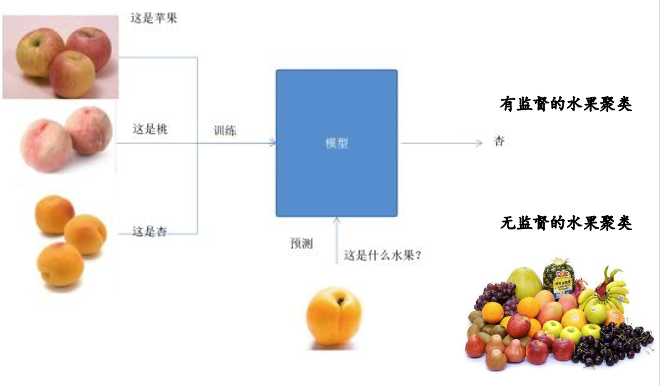
\includegraphics[width=1\textwidth]{figs/监督与无监督.png}
\caption{监督学习与无监督学习的异同点}
\label{监督学习与无监督学习的异同点}
\end{figure}

\subsection{半监督学习 (Semi-Supervised Learning)} 

半监督学习介于监督学习与无监督学习之间，适用于只有部分数据被标注的场景。在许多实际应用中，标注数据往往稀缺且成本较高，因此半监督学习结合了大量未标注数据和少量标注数据来进行训练。其核心目标是利用未标注数据中的潜在信息，提升模型的泛化能力，从而在标注数据不足的情况下取得更好的性能。

在半监督学习中，通常借助无监督学习的方法来从未标注数据中挖掘结构信息，如聚类和数据分布的特征等。常见的半监督学习方法包括自训练（self-training）、生成模型（如生成对抗网络，GAN）以及图模型等。这些方法通过不同的策略利用未标注数据，以增强模型对数据特征的学习。

半监督学习（Semi-supervised Learning）的方式，既用到了标签数据，又用到了非标签数据。
从这个角度来看，现代人类成长学习的最佳方式当属“半监督学习”！它既不是纯粹的“监督学习”（因为如果完全是这样，就会扼杀我们的创造力和认知体系，也就永远不可能超越我们的父辈和师辈），也不属于完全的“非监督学习”，因为如果完全这样，我们会如无根之浮萍，会花很多时间重造轮子。前人的思考，我们的阶梯。

事实上，半监督学习就是以“已知之认知（标签化的分类信息）”，扩大“未知之领域（通过聚类思想将未知事物归类为已知事物）”。

但这里隐含了一个基本假设—聚类假设（Cluster Assumption），其核心要义就是：相似的样本，拥有相似的输出。

半监督学习广泛应用于图像分类、语音识别、文本分类等领域，尤其在这些任务中，标注数据的获取成本较高。通过半监督学习，模型可以在有限的标注数据上进行有效训练，并利用未标注数据进一步提高学习效果，减少对大量标注数据的依赖。

 

%\begin{table}[htbp]
%\centering
%\begin{tabular}{|c|c|c|c|c|c|}
%\hline
%{\bf 学习范式} & {\bf 训练样本} & 优化目标 &学习准则 & {\bf 反馈方式} & {\bf 适用场景} \medskip \\
%\hline
%监督学习 & 标注好的 $(X, Y)$ 数据 & $y=f({\bf x})$ 或 $p(y|{\bf x})$ & 期望风险最小化  最大似然估计 & 明确的目标值 & 分类、回归、生成任务   \\
%\hline
%无监督学习 &  无标注的 $X$ 数据& $p({\bf x})$ 或带隐变量~${\bf z}$的$p({\bf x}|{\bf z})$ &  最大似然估计 最小重构错误  & 隐含的模式或结构   &数据聚类、降维、分布估计  \\
%\hline
%强化学习 & %环境状态 $S$ 和动作 $A$，
%智能体和环境交互的轨迹~$\tau$ 和累积奖励~$G_\tau$  & 期望总回报 $\mathbb{E}_\tau(G_\tau)$ &策略评估 策略改进  & 延迟的奖励信号 $R$   & 决策优化、策略学习   \\
%\hline
%\end{tabular}
%\caption{监督学习、无监督学习、强化学习对比}
%\label{tab:3learning}
%\end{table}

\begin{table}[htbp]
\centering
\caption{监督学习、无监督学习、强化学习对比}
\begin{tabular}{|c|c|c|c|
}
\hline
{\bf 学习范式} & {\bf  监督学习} & {\bf 无监督学习} & {\bf 强化学习} \\
\hline
{\bf 训练样本} &  标注好的 $(X, Y)$ 数据  &  无标注的 $X$ 数据  &%环境状态 $S$ 和动作 $A$，
智能体和环境交互的轨迹~$\tau$ 和累积奖励~$G_\tau$  
 \\
\hline
{\bf 优化目标}  &  $y=f({\bf x})$ 或 $p(y|{\bf x})$  & $p({\bf x})$ 或带隐变量~${\bf z}$的$p({\bf x}|{\bf z})$ & 期望总回报 $\mathbb{E}_\tau(G_\tau)$ 
 \\
\hline
{\bf 学习准则} &  期望风险最小化、最大似然估计  & 最大似然估计、最小重构错误 & 策略评估、策略改进   \\
\hline
 {\bf 反馈方式}  & 明确的目标值  &隐含的模式或结构   &延迟的奖励信号 $R$   \\
\hline
  {\bf 适用场景} & 分类、回归、生成任务 &  数据聚类、降维、分布估计&决策优化、策略学习 \\
\hline
\end{tabular}
\label{tab:3learning}
\end{table}


%{\bf 结合场景的选择}
%
%
%机器学习范式的选择直接影响问题的建模方式和解决方案的设计。监督学习适用于有标注数据的任务，半监督学习通过结合未标注数据来弥补标签的不足，无监督学习则通过挖掘数据的内在结构来发现潜在的规律，而强化学习则适用于动态决策问题，依赖环境的反馈进行学习和优化。通过理解不同范式的特点及应用场景，能够帮助我们更好地选择适合的机器学习方法，解决实际问题。
 %---


\subsection{传统机器学习的辉煌与局限}
在机器学习的发展过程中，监督学习、无监督学习和和半监督学习是机器学习的三大经典范式，构成了传统机器学习的核心。

这三大范式各自对应不同的应用场景与需求。
如果任务可以明确量化输入与输出之间的映射关系且有足够标注数据，监督学习是首选。但是，监督学习的人工标注成本非常高，尤其是在需要大量高质量标注数据的复杂任务中，这一问题尤为显著。在缺乏标注但数据量庞大的场景，无监督学习有助于发现数据的潜在结构。
而在标注数据稀缺的情况下，半监督学习通过结合少量标注数据和大量未标注数据，显著提升了模型的泛化能力。

这些方法为机器学习奠定了坚实的理论和技术基础，并在实际应用中大放异彩，例如图像分类、语音识别、文本分析等任务中。

然而，传统机器学习也有其不可忽视的局限性：

1. 标注数据依赖

监督学习依赖大量人工标注的数据，而这些数据的获取过程昂贵且耗时。例如，图像分类需要手工为每张图片标注类别，语音识别需要逐句转录文本。这种对标注数据的强烈依赖限制了监督学习在大规模场景中的应用。

2. 无法高效利用未标注数据
无监督学习虽然能够从未标注数据中挖掘结构信息，但其目标和反馈信号较为模糊，效果往往不如监督学习直观明确。在许多情况下，未标注数据的潜力未被充分挖掘。

3. 对复杂问题的处理能力有限
传统的机器学习方法在面对高维复杂数据（如视频、图像生成）或动态决策问题（如游戏对弈、机器人控制）时，表现出较大的不足。

\section{从生物学启发到机器学习的新方向}
在本章中，我们介绍了三种主要的机器学习范式：监督学习、无监督学习和强化学习。每种范式都有其独特的应用场景和优势，但它们也存在各自的局限性。

{\em (需修改) 为了更好地理解这些范式的优势和瓶颈，我们可以借鉴生物学中大脑学习的方式，特别是神经系统如何在缺乏完全监督信号的情况下高效地学习。这些生物学的启示不仅能帮助我们突破当前机器学习中的限制，还能引领我们探索新的学习策略和技术方向。

人类大脑是一个高度复杂的计算系统，约由~${10}^{14}$  个神经元突触组成。每个神经元通过突触与其他神经元相互连接，形成庞大而复杂的网络。这种巨大的连接数使得大脑能够在多样化的任务中迅速学习并适应环境变化。
这一数量级的突触连接对应着机器学习模型中的大规模参数，其调整需要大规模的计算和优化过程。

然而，人类大脑也受到两个关键的生物数量级的限制：神经元突触的数量和生命的时间长度。%\cite{Hinton}

1. 突触数量与参数优化的挑战

大量突触连接意味着需要对庞大的参数空间进行调整。类似于神经网络中的权重参数，大脑需要通过突触优化其连接来提升认知效率。然而，单纯依赖监督信号进行调整并不现实，因为监督信号的获取往往稀缺且成本高昂。

2. 生命时间的限制

人类的生命长度大约为 $10^9$ 秒，这意味着在有限的时间内，大脑必须高效地学习并调整其连接。如果每个突触的调整都依赖于外部监督信号（例如人工标注的数据），学习所需的时间将远远超过实际可用的生命时间。

基于上述生物学的观察，Hinton 提出了一个重要的观点：{\bf 生物大脑无法完全依赖外部监督信号这种低效的学习方式，特别是在监督信号稀缺且成本高昂的情况下，而是必须通过其他机制来高效地进行学习}。
为了满足生存和适应环境的需求，生物大脑更依赖于无监督学习和自监督学习，从环境中获取丰富的信息，并通过这些信息建立内在模型。例如，观察世界、模仿行为、通过互动学习规律。
这些模型不仅帮助人类在没有标签的情况下理解世界，还能通过模仿和互动来不断优化学习过程。例如，通过观察他人的行为、与环境互动，或在无监督的情况下提取数据中的规律。


Hinton 的生物学启示为机器学习领域提供了重要的思路。在当前的研究中，依赖人工标注数据的监督学习方法面临诸多挑战，未来的研究应当更加关注如何利用未标注数据进行高效的学习。无监督学习、自监督学习和半监督学习为解决这一问题提供了有效的途径。未来的人工智能系统，将更加接近生物大脑的学习机制，能够像人类一样主动从环境中获取知识，并通过不断的互动和自我调整，提升学习效率和适应能力。这些生物学的启发不仅为机器学习的发展提供了新思路，也将推动人工智能技术的不断进步。}


%机器学习中的启示：
%监督学习的局限性：
%
%人工标注不仅昂贵，而且难以覆盖多样化的现实场景。
%某些任务（如语言模型、大规模图像生成）所需的标注数据量极其庞大，难以完全依赖人工标注。
%发展方向：
%
%无监督学习：利用未标注数据，挖掘数据中的潜在模式和结构。
%自监督学习：通过设计任务（如预测未见部分、填补缺失内容等），在无标注数据上生成训练信号。例如，BERT 使用了“掩盖词预测”任务，DALL-E 利用“图像-文本匹配”任务。
%半监督学习：结合少量标注数据和大量未标注数据，降低标注成本。
%
%Hinton 的观点提醒我们，在生物与人工智能中，完全依赖监督信号的学习方式不仅不现实，也效率低下。未来的研究应更多关注如何高效地利用无标注数据，让模型像人类一样从环境中主动学习，进一步提升学习效率和适应能力。
%

%机器学习中的启示
%从生物学的视角出发，我们能够对现有机器学习范式的局限性有更深入的理解。特别是在监督学习中，人工标注数据的获取既困难又昂贵，且在面对复杂的现实世界时，这种标注方法往往无法满足需求。因此，机器学习领域正在朝着无监督学习和自监督学习的方向发展，力图在没有大量标注数据的情况下，实现高效的学习。
%
%无监督学习：无监督学习不依赖人工标注，而是通过分析未标注数据的结构和模式来进行学习。例如，聚类和降维技术可以帮助我们揭示数据的内在规律，而不需要依赖标签信息。这种方法为处理海量未标注数据提供了可行的解决方案。
%
%自监督学习：自监督学习通过设计预定任务来生成学习信号，使得模型能够从未标注数据中进行自我学习。常见的自监督学习方法包括语言模型中的“掩盖词预测”任务和图像生成中的“图像-文本匹配”任务。这些方法能够帮助模型从复杂数据中自动提取有用信息，从而构建更为精确的内在模型。
%
%半监督学习：半监督学习结合了少量标注数据与大量未标注数据，旨在利用标注数据提高模型的精度，同时最大限度地减少标注数据的需求。通过这种方式，半监督学习能够在减少标注成本的同时，提升模型的性能和泛化能力。

\nocite{*}
\printbibliography[heading=bibintoc, title=\ebibname]

\newpage